% main.tex -- "Proof != Execution" (W25 lead writer, final paper wave, CONTRACT §13).
% Claims are governed by ../lit/pass2/NOVELTY_UPDATE.md; every number is a numbers.tex macro.
\documentclass[sigconf,anonymous,review]{acmart}

% macros.tex -- notation shared by all sections (W2).
\usepackage{xcolor}
\usepackage{xspace}
\usepackage{enumitem}
% Long monospace header names otherwise overrun the narrow sigconf column.
\setlength{\emergencystretch}{2em}

% Placeholder for any number that is not yet measured. Never replace by hand
% with a guess: numbers.tex is filled from analysis outputs only.
\newcommand{\TBD}[1]{\textcolor{red}{\textbf{[TBD:\allowbreak #1]}}}
\newcommand{\todo}[1]{\textcolor{orange}{[TODO: #1]}}

% Protocol claims and fields
\newcommand{\clm}[1]{\texttt{#1}}
\newcommand{\htm}{\clm{htm}\xspace}
\newcommand{\htu}{\clm{htu}\xspace}
\newcommand{\ath}{\clm{ath}\xspace}
\newcommand{\jti}{\clm{jti}\xspace}
\newcommand{\iat}{\clm{iat}\xspace}
\newcommand{\cnf}{\clm{cnf}\xspace}
\newcommand{\jkt}{\clm{cnf.jkt}\xspace}
\newcommand{\hdr}[1]{\texttt{#1}}

% Parties and adversaries
\newcommand{\Cl}{\mathsf{C}}
\newcommand{\Ver}{\mathsf{V}}
\newcommand{\PDP}{\mathsf{P}}
\newcommand{\Exe}{\mathsf{E}}
\newcommand{\Aleak}{\ensuremath{\mathcal{A}_{\mathrm{leak}}}\xspace}
\newcommand{\Aclient}{\ensuremath{\mathcal{A}_{\mathrm{client}}}\xspace}

% Views, executions, sets
\newcommand{\view}{v}
\newcommand{\exe}{x}
\newcommand{\op}{\mathit{op}}
\newcommand{\Acc}{\mathsf{Acc}}
\newcommand{\res}{\mathsf{res}}
\newcommand{\canon}{\mathsf{canon}}
\newcommand{\Cov}{\mathsf{Cov}}
\newcommand{\Req}{\mathcal{R}}

% Failure classes, hypotheses
\newcommand{\GA}{\textsf{G1}\xspace}
\newcommand{\GB}{\textsf{G2}\xspace}
\newcommand{\GC}{\textsf{G3}\xspace}
\newcommand{\Hyp}[1]{\textsf{H#1}\xspace}
\newcommand{\Exp}[1]{\textsf{E#1}\xspace}
\newcommand{\Abl}[1]{\textsf{A#1}\xspace}

% Figures (Fig. 1 views, Fig. 2 harness) are TikZ, drawn in the .tex sources.
\usepackage{tikz}
\usetikzlibrary{arrows.meta,positioning,fit,calc,backgrounds}

% acmart provides the definition environment (acmthm).

% numbers.tex -- every quantitative claim in the paper is a macro defined here.
% All values filled (W20, 2026-11-24) from experiments/{defence,ablation}/REPORT.md and disclosure/TRIAGE.md.
% Fill ONLY from recorded outputs (harness/logs/*, prevalence/*), and cite
% the producing script next to each value. Never estimate.

% --- Harness components (built and tested; NOT campaign results) ---
% Gateways implemented, rendered and smoke-tested: harness/gateways/README.md "Pinned images"
% table (6 rows); harness/orchestrator/SMOKE.md: 36/36 PASS rows (18 stub verifier + 18 real verifier).
\newcommand{\NumGateways}{6}
\newcommand{\NumGatewayProfiles}{3}            % gateways/README.md "What the profiles mean"
\newcommand{\NumSmokePass}{36}                 % orchestrator/SMOKE.md, count of "| PASS |" rows
\newcommand{\NumSmokeRuns}{36}                 % same file, 0 FAIL rows
% Executors implemented and conformance-tested: executors/conformance/results_A.md (4) +
% executors/{spring,aspnet,rails,laravel}/CONFORMANCE.md (4).
\newcommand{\NumFrameworks}{8}
\newcommand{\NumBenchOps}{13}                  % mutator/README.md L5 (base_ops.py: 13 canonical operations)
\newcommand{\NumBenchOpIds}{17}                % executors/conformance/README.md "Required checks" 1 (17 op_ids)
\newcommand{\NumConformanceCases}{23}          % same, 23 cases
\newcommand{\NumVerifierTests}{125}            % verifier/README.md L100: 125 passed, 0 failed
% Primitive catalogue: harness/mutator/README.md L13-14 (84 = G1 37 + G2 32 + G3 15);
% re-counted from primitives/{g1,g2,g3}.yaml "id:" lines on 2026-11-23 (37/32/15).
\newcommand{\NumPrimitives}{84}
\newcommand{\NumPrimitivesGOne}{37}
\newcommand{\NumPrimitivesGTwo}{32}
\newcommand{\NumPrimitivesGThree}{15}
% Planned matrix: orchestrator/README.md L56-57 (6 gw x 3 profiles x 3 placements x 8 fw x 2 override).
\newcommand{\NumMatrixTopologies}{864}
\newcommand{\NumPlacements}{3}               % CONTRACT.md §5 (edge, origin, both)
\newcommand{\NumPilotTopologies}{24}           % orchestrator/README.md L59
\newcommand{\NumDepthOneCasesPilot}{948}       % runner/README.md L55-56: depth-1 cases, fastapi pilot, 0 transport errors

% --- Scope of the binding (A_leak) campaign: four experiments, all --stubs off, 2026-11-23 ---
% Per-experiment rows: kill/G1_REPORT.md §1; ext-gw/REPORT.md §1; ext-fw/REPORT.md §1;
% ext-routes/REPORT.md §1. Totals recomputed by paper/figs/make_figs.py -> figs/aggregate.json
% ("leak_total", "leak"), from experiments/*/analysis/{hits_per_topology.csv,hits_all.jsonl,resolution.csv}.
\newcommand{\NumTopologies}{256}               % aggregate.json leak_total.topologies = 48+96+80+32
\newcommand{\NumTopoKill}{48}                  % kill/G1_REPORT.md L3
\newcommand{\NumTopoExtGw}{96}                 % ext-gw/REPORT.md L3
\newcommand{\NumTopoExtFw}{80}                 % ext-fw/REPORT.md L3 (48 edge + 32 A3)
\newcommand{\NumTopoExtFwEdge}{48}             % ext-fw/REPORT.md L4-5
\newcommand{\NumTopoExtFwAThree}{32}           % ext-fw/REPORT.md L6-8
\newcommand{\NumTopoExtRoutes}{32}             % ext-routes/REPORT.md "Data"
\newcommand{\NumTopoVOneEdge}{192}             % 48+96+48: full 6 gw x 8 fw x 2 profiles x 2 override grid (aggregate.json heatmap_cells_full=48 cells x 4)
\newcommand{\NumCasesVOne}{948}                % depth-1 cases per v1 topology, kill/G1_REPORT.md L3
\newcommand{\NumCasesVTwo}{581}                % depth-1 cases per v2 topology, ext-routes/REPORT.md "Data"
\newcommand{\NumCases}{230{,}944}              % 45,504 + 91,008 + 75,840 + 18,592 (the four "cases sent" rows)
\newcommand{\NumCasesKill}{45{,}504}         % kill/G1_REPORT.md §1
\newcommand{\NumCasesExtGw}{91{,}008}          % ext-gw/REPORT.md §1
\newcommand{\NumCasesExtFw}{75{,}840}          % ext-fw/REPORT.md §1
\newcommand{\NumCasesExtRoutes}{18{,}592}      % ext-routes/REPORT.md §1
\newcommand{\NumTransportErrors}{2}            % ext-gw/REPORT.md §1 (2 non-hit cases); 0 in kill, ext-fw, ext-routes
\newcommand{\NumTopologiesAll}{352}            % \NumTopologies + \NumEFourTopologies (256 + 96)
\newcommand{\NumCasesAll}{233{,}728}           % \NumCases + \NumEFourCases (230,944 + 2,784)
\newcommand{\NumNewRoutes}{4}                  % ext-routes/REPORT.md route table (postAccount, getStatements, deleteStatement, catchAllFile)
% --- E1 prevalence: binding/prevalence/E1_results.md (W8), file:line given per macro ---
\newcommand{\NumSpecFiles}{4{,}138}            % E1_results.md L28
\newcommand{\NumSpecFilesParsed}{4{,}105}      % L28
\newcommand{\NumSpecFilesFailed}{33}           % L28
\newcommand{\NumSpecs}{2{,}652}                % L29 (APIs with >=1 parsed version; denominator)
\newcommand{\NumOps}{127{,}642}                % L31
\newcommand{\NumStateChangingOps}{66{,}184}    % L31
\newcommand{\NumApisWithStateOps}{2{,}063}     % L39
\newcommand{\NumApisCollided}{234}             % L39
\newcommand{\PctApisCollided}{8.8\%}           % L39, 95% Wilson CI [7.8, 10.0]
\newcommand{\CIApisCollided}{[7.8, 10.0]}
\newcommand{\NumStateOpsCollided}{7{,}577}     % L39
\newcommand{\PctUnderBound}{11.4\%}            % L39, state-changing ops in collided keys
\newcommand{\CIUnderBound}{[11.2, 11.7]}       % L39
\newcommand{\NumSpecsNonAWS}{2{,}298}          % L40
\newcommand{\NumApisCollidedNonAWS}{66}        % L40
\newcommand{\PctApisCollidedNonAWS}{2.9\%}     % L40, CI [2.3, 3.6]
\newcommand{\CIApisCollidedNonAWS}{[2.3, 3.6]}
\newcommand{\NumStateOpsNonAWS}{54{,}552}      % L40
\newcommand{\NumStateOpsCollidedNonAWS}{197}   % L40
\newcommand{\PctUnderBoundNonAWS}{0.4\%}       % L40, CI [0.3, 0.4]
\newcommand{\NumSpecsNonHyper}{1{,}329}        % L41 (excl. amazonaws/azure/googleapis/microsoft)
\newcommand{\NumApisCollidedNonHyper}{47}      % L41
\newcommand{\PctApisCollidedNonHyper}{3.5\%}   % L41, CI [2.7, 4.7]
\newcommand{\NumStateOpsCollidedNonHyper}{149}   % L41
\newcommand{\PctUnderBoundNonHyper}{0.5\%}     % L41 (149 of 29,700), CI [0.4, 0.6]
\newcommand{\NumSpecsFinance}{106}             % L42
\newcommand{\NumApisCollidedFinance}{4}        % L42
\newcommand{\PctApisCollidedFinance}{3.8\%}     % L42, CI [1.5, 9.3]
\newcommand{\NumStateOpsFinance}{2{,}404}      % L42
\newcommand{\NumStateOpsCollidedFinance}{9}    % L42
\newcommand{\PctUnderBoundFinance}{0.4\%}      % L42, CI [0.2, 0.7]
\newcommand{\NumStateOpsCloud}{16{,}843}       % L65
\newcommand{\NumStateOpsCollidedCloud}{7{,}407}% L65
\newcommand{\PctUnderBoundCloud}{44.0\%}       % L65, CI [43.2, 44.7]
\newcommand{\NumMOneOps}{9{,}227}              % L49 (M1 flagged ops)
\newcommand{\NumMOneOpsAWS}{9{,}102}           % L49
\newcommand{\NumEcTwoOpsPerKey}{594}           % L117 (EC2 ops on each of POST / and GET /)
\newcommand{\NumApisDocOverride}{6}            % L58 (all Amadeus), 0.2% [0.1, 0.5]
\newcommand{\PctApisDocOverride}{0.2\%}
% Precision (T9), E1_results.md L89-96; seeded stratified sample, seed 20261123 (L79)
\newcommand{\NumValidationSample}{100}         % L79
\newcommand{\PrecMOne}{1.00}                   % L89: 30/30, CI [0.89, 1.00]
\newcommand{\NumMOneTP}{30}                  % L89
\newcommand{\NumMOneSample}{30}              % L89
\newcommand{\NumMFiveFlags}{3}               % L53/L92 (M5 population = 3)
\newcommand{\PrecMTwo}{0.40}                   % L90: 12/30, CI [0.25, 0.58]
\newcommand{\PrecMFour}{0.30}                  % L91: 11/37 (+1 unclear counted FP), CI [0.17, 0.46]
\newcommand{\PrecMFive}{0.67}                  % L92: 2/3, CI [0.21, 0.94]
\newcommand{\PrecWeighted}{0.986}              % L94: stratum-weighted, ~9,289 true flagged ops
\newcommand{\PrecNonMOneWeighted}{0.32}        % L96: ~62 true flagged ops
\newcommand{\NumFinanceTP}{4}                  % L100: 4 of 9 flagged finance ops TP
\newcommand{\NumFinanceFlagged}{9}             % L100
\newcommand{\NumFinanceApisTP}{2}              % L100: in 2 of 106 finance APIs
\newcommand{\NumConfirmedApis}{44}             % L111: hand-confirmed lower bound
\newcommand{\NumConfirmedApisAWS}{25}          % L111
\newcommand{\NumConfirmedApisNonAWS}{19}       % L111
\newcommand{\PctConfirmedApisNonAWS}{0.8\%}    % L111 (19 of 2,298)
\newcommand{\PctUnderBoundAllFiles}{9.6\%}     % L125 sensitivity, every parsed file
\newcommand{\PctUnderBoundAllFilesNonAWS}{0.3\%}% L126
\newcommand{\NumFhirTypesConditional}{146}     % L149: 146/146 HAPI R4 resource types
\newcommand{\NumMcpDpopMentions}{0}            % L159

% --- E2 framework survey: binding/prevalence/E2_results.md (W8) ---
\newcommand{\NumPinnedSourcesVerified}{20}     % E2_results.md L3: 20/20 byte-identical
\newcommand{\NumDocChecks}{19}                 % L3: 19/19 phrases found
\newcommand{\NumTargetFrameworks}{8}           % L47 ("eight target frameworks")
\newcommand{\NumOverrideFrameworks}{2}         % L47: default-on (Rails unless api_only; Laravel always)
\newcommand{\NumOptInFrameworks}{3}            % L50: Spring Boot, ASP.NET Core, Express
\newcommand{\NumNoOverrideFrameworks}{3}       % L51: FastAPI/Starlette, Django, Go
\newcommand{\PctEnableSpring}{0.99\%}          % L107: 7,168 / 721,920
\newcommand{\PctEnableAspnet}{0.06\%}          % L109: 225 / 383,488
\newcommand{\PctEnableExpress}{1.87\%}         % L110: 69,760 / 3,727,360
\newcommand{\PctEnableExpressNpm}{1.11\%}      % L112: npm downloads 9,415,448 / 845,699,176
\newcommand{\PctExpressQueryGetter}{52.9\%}    % L113: 22,880 / 43,264
\newcommand{\PctEnableGorilla}{1.15\%}         % L114: 98 / 8,496
\newcommand{\PctRailsApiOnly}{13.9\%}          % L115: 26,240 / 188,416
\newcommand{\PctRailsOverrideOn}{86\%}         % L115 (approx., complement of api_only)
\newcommand{\PctSymfonyParamOn}{36.7\%}        % L116: 3,128 / 8,520

% --- Binding-soundness findings (A_leak). Totals: figs/aggregate.json "leak_total" ---
\newcommand{\NumHits}{2{,}968}                 % 680 + 1,368 + 694 + 226 (§1 of each report)
\newcommand{\NumHitsKill}{680}                 % kill/G1_REPORT.md §1
\newcommand{\NumHitsExtGw}{1{,}368}            % ext-gw/REPORT.md §1
\newcommand{\NumHitsExtFw}{694}                % ext-fw/REPORT.md §1
\newcommand{\NumHitsExtRoutes}{226}            % ext-routes/REPORT.md §1
\newcommand{\NumHitsGOneOracle}{2{,}582}       % aggregate.json leak_total.oracle_g1 (label of the primitive)
\newcommand{\NumHitsGTwoOracle}{386}           % aggregate.json leak_total.oracle_g2
\newcommand{\NumHitsRCSeven}{36}               % oracle-g2 hits whose ddmin witness is one byte in ?op= (kill RC7 8, ext-gw §7 12, ext-fw §6 16)
\newcommand{\NumHitsGOne}{2{,}618}             % aggregate.json leak_total.mech_g1 (= oracle g1 + RC7)
\newcommand{\NumHitsGTwo}{350}                 % aggregate.json leak_total.mech_g2 (kill 24, ext-gw 168, ext-fw 48, ext-routes 110)
\newcommand{\NumHitsGThree}{0}                 % G3 binding hits: 0 in all four reports
\newcommand{\NumSOneHits}{1{,}687}             % aggregate.json leak_total.S1
\newcommand{\NumSTwoHits}{1{,}281}             % aggregate.json leak_total.S2 (S3 = 0)
\newcommand{\NumConfirmedHits}{2{,}284}        % rerun 3x on fresh topologies: 680 + 684 + 694 + 226
\newcommand{\NumConfirmedExtGw}{684}           % ext-gw/REPORT.md §1: default profile; recommended byte-identical
\newcommand{\NumFlaky}{0}                      % all four reports: 0 flaky, 0 irreproducible
\newcommand{\NumBZero}{0}                      % B0 verifier bypass, all four reports
\newcommand{\NumVulnTopologies}{230}           % topologies with res_hat > 1 (resolution.csv, all four); the 26 others: 24 A3 artefacts (ext-fw §A3.2-3) + 2 aspnet v2 ovoff
\newcommand{\NumGTwoTopologies}{68}            % topologies with >= 1 G2 (mechanism) hit: kill 4, ext-gw 28, ext-fw 8, ext-routes 28
\newcommand{\NumResPairs}{3{,}168}             % (topology, base op) pairs: 624 + 1,248 + 1,040 + 256
\newcommand{\NumResOne}{2{,}421}               % aggregate.json leak_res_hat_total
\newcommand{\NumResTwo}{268}
\newcommand{\NumResThree}{446}
\newcommand{\NumResFour}{28}
\newcommand{\NumResFive}{3}
\newcommand{\NumResSix}{2}
\newcommand{\MaxResolution}{6}                 % ext-routes/REPORT.md §4 (getAccount/updateAccount/deleteAccount)
\newcommand{\MaxResolutionVOne}{4}             % kill §4, ext-gw §4 (v1 route space)
% G2 mechanisms (binding soundness)
\newcommand{\NumHitsFragPath}{144}             % '#' in path, v1: nginx 24 (kill RC6) + 48 (ext-fw) + Kong 72 (ext-gw RC-W13-B)
\newcommand{\NumHitsFragAll}{198}             % B1 total: v1 '#'-in-path 144 + ext-routes X1 12 + X2 42
\newcommand{\NumGTwoKill}{24}                  % kill RC6 (aggregate.json leak.kill.mech_class.g2)
\newcommand{\NumGTwoExtGw}{168}                % ext-gw §1 "genuine G2 after ddmin"
\newcommand{\NumGTwoExtFw}{48}                 % ext-fw edge g2 64 minus 16 fragment-in-query (aggregate.json)
\newcommand{\NumGTwoExtRoutes}{110}            % ext-routes §1
\newcommand{\NumHitsFragKong}{72}              % ext-gw/REPORT.md §1
\newcommand{\NumHitsApisixPct}{96}             % ext-gw/REPORT.md §1, RC-W13-A
\newcommand{\NumFwApisixPct}{4}                % ext-gw RC-W13-A: aspnet, express, go-chi, rails
\newcommand{\NumHitsXOne}{12}                  % ext-routes §1: fragment nested-route (operation change)
\newcommand{\NumHitsXTwo}{42}                  % ext-routes §1: fragment id suffix
\newcommand{\NumHitsXThree}{56}                % ext-routes §1: dot-segment catch-all
\newcommand{\NumFwXThree}{7}                   % ext-routes §0: 7 of 8 frameworks (not aspnet)
\newcommand{\NumFragServers}{3}                % uvicorn/h11, Go net/http, FrankenPHP (ext-fw §0, ext-routes X1)
\newcommand{\NumHitsOverrideVTwo}{116}         % ext-routes §1: G1 method override (X4+X5)
\newcommand{\NumLatentDot}{468}                % kill/ROOT_CAUSES.md L1: allow -> 404 per v1 matrix (nginx, envoy default)
% A3 placement (ext-fw/REPORT.md §A3)
\newcommand{\NumHitsEnvoyOrigin}{90}           % §1 / §A3.1: envoy-origin, 8 frameworks, all G1
\newcommand{\NumHitsNginxOriginFixed}{105}     % §A3.2 table (26+17+10+11+11+11+9+10), all confirmed 3/3
\newcommand{\NumJtiReplayEnvoyBoth}{606}       % §A3.3: 606/948 jti_replay on envoy-both
\newcommand{\NumBindingGTwoClasses}{3}       % GATE_DECISION.md binding-soundness table (B1 '#', B2 APISIX %2f, B3 dot-segment catch-all)
% Disclosure drafts: disclosure/TRIAGE.md L20-21 (1 NEW: APISIX RC-W13-A; 3 KNOWN-UNFIXED: '#' in uvicorn-h11,
% Go net/http, FrankenPHP) and L26 ("Drafts written for the 1 NEW + 3 KNOWN-UNFIXED items ... No report is sent").
\newcommand{\NumDisclosures}{4}
\newcommand{\NumDisclosuresNew}{1}             % TRIAGE.md L20 -- NOT used in the paper: NOVELTY_UPDATE.md §C3 reclassifies APISIX RC-W13-A as a CVE-2026-124680 variant
\newcommand{\NumDisclosuresKnown}{3}           % TRIAGE.md L21
\newcommand{\NumDisclosuresDocumented}{6}      % TRIAGE.md L22 (documented behaviour, no report)

% --- E4 authorization soundness (A_client + PDP): e4/REPORT.md, e4/ROOT_CAUSES.md (W12) ---
% Totals recomputed from e4/runs/summary.csv by figs/make_figs.py -> aggregate.json "e4".
\newcommand{\NumEFourTopologies}{96}           % REPORT.md L12; summary.csv 96 rows
\newcommand{\NumEFourCells}{144}              % REPORT.md §13: full 6 gw x 2 policies x 2 profiles x 6 fw
\newcommand{\NumEFourVectors}{29}              % REPORT.md §3
\newcommand{\NumEFourCases}{2{,}784}           % summary.csv sum(cases) = 96 x 29
\newcommand{\NumEFourViolations}{325}          % REPORT.md §5
\newcommand{\NumEFourVulnTopologies}{50}       % REPORT.md L12
\newcommand{\NumEFourAdmin}{180}               % summary.csv sum(admin)
\newcommand{\NumEFourBob}{145}                 % summary.csv sum(bob)
\newcommand{\NumEFourClasses}{7}               % REPORT.md §6
\newcommand{\NumEFourComponents}{5}            % REPORT.md §6 (ASP.NET, Express, Spring, Rails, Kong)
\newcommand{\NumEFourAllowBreak}{2}            % REPORT.md §6, RC1 + RC2
\newcommand{\NumEFourHtuMismatch}{148}         % REPORT.md §5
\newcommand{\NumEFourReruns}{7}                % REPORT.md §7: one topology per class, 3 reps each
% per class: n_topo / n_viol (REPORT.md §6 table)
\newcommand{\EFourRCOneTopo}{10}\newcommand{\EFourRCOneViol}{76}
\newcommand{\EFourRCTwoTopo}{16}\newcommand{\EFourRCTwoViol}{144}
\newcommand{\EFourRCThreeTopo}{12}\newcommand{\EFourRCThreeViol}{24}
\newcommand{\EFourRCFourTopo}{6}\newcommand{\EFourRCFourViol}{12}
\newcommand{\EFourRCFiveTopo}{12}\newcommand{\EFourRCFiveViol}{36}
\newcommand{\EFourRCSixTopo}{4}\newcommand{\EFourRCSixViol}{12}
\newcommand{\EFourRCSevenTopo}{7}\newcommand{\EFourRCSevenViol}{21}
% native ACLs (REPORT.md §9)
\newcommand{\NumNativeNginx}{2}
\newcommand{\NumNativeEnvoyRaw}{13}
\newcommand{\NumNativeEnvoyNorm}{9}

% --- Ablations produced by W17/W18 (A1/A4/A5 filled by W18 from experiments/ablation/) ---
% A1 (W18): experiments/ablation/REPORT.md §A1; analysis/a1_variant_summary.csv, a1_runs_swap_variant_summary.csv,
% legit/runs/*/legit.jsonl. nginx default edge x {fastapi,spring,rails,laravel}:v2 x override, 1239 cases/topology.
\newcommand{\AblOneTopos}{64}\newcommand{\AblOneCases}{1{,}239}\newcommand{\AblOneSwapCases}{357}
\newcommand{\AblOneHitsFull}{192}       % = no-htm = no-ath = digest-nogate (identical hit sets)
\newcommand{\AblOneHitsNoHtu}{432}\newcommand{\AblOneResNoHtu}{10}\newcommand{\AblOneResFull}{6}
\newcommand{\AblOneHitsQuery}{147}      % -45: query dispatch 40 + ?_method 5
\newcommand{\AblOneHitsDigest}{129}     % -63, with the body-check hop; digest-nogate = 192
\newcommand{\AblOneHitsQueryDigest}{84} % residual: header override 18, content-type 2, '#' 48, dot-segment 16
\newcommand{\AblOneGTwoSurvive}{60}     % G2 hits, unchanged in every binding variant
\newcommand{\AblOneSwapNoHtm}{192}\newcommand{\AblOneSwapNoHtu}{720}\newcommand{\AblOneSwapFull}{0}
\newcommand{\AblOneLegitN}{18}\newcommand{\AblOneLegitFRNginx}{0}
\newcommand{\AblOneLegitFRHapExact}{4}\newcommand{\AblOneLegitFRHapRfc}{2}\newcommand{\AblOneLegitFRHapSorted}{0}
\newcommand{\AblOneResult}{htm, htu and ath ablated and query/body binding added (\AblOneTopos{} topologies): \AblOneHitsFull{} hits with full binding; dropping htu gives \AblOneHitsNoHtu{} (and \AblOneSwapNoHtu{} cross-op replays), dropping htm \AblOneSwapNoHtm{} method-swap replays; query binding gives \AblOneHitsQuery{}, body binding (with a body-checking hop) \AblOneHitsDigest{}, both \AblOneHitsQueryDigest{}; all \AblOneGTwoSurvive{} G2 hits survive every variant}
% A2 (W17): experiments/defence/REPORT.md §4, analysis/a2_tables.md (scripts/a2_ablation.py; offline
% D-B decision replay, 472/472 agreement with the live D-B runs)
\newcommand{\AblTwoResult}{the percent-encoder is load-bearing (without it all 28 \texttt{\#} and 8 of 12
dot-segment witnesses return); method binding closes the 31 override witnesses; case- and slash-preserving
comparison close the \NumEFourCaseSlash{} E4 case-fold and \texttt{//} violations; dot removal and the prefix map
reopen nothing}
\newcommand{\NumEFourCaseSlash}{10}            % a2_tables.md: E4 case 4 + dslash 6
% A4 (W18): REPORT.md §A4; analysis/a4_binding_family_loo.csv, a4_e4_family_loo_merged.csv (existing data only)
\newcommand{\AblFourHits}{2{,}968}\newcommand{\AblFourGOneShare}{87.0\%}\newcommand{\AblFourGTwoShare}{13.0\%}
\newcommand{\AblFourFamiliesWithHits}{9}\newcommand{\AblFourFamilies}{29}
\newcommand{\AblFourFragGTwoShare}{56.6\%}\newcommand{\AblFourDotsegEFourShare}{67.7\%}
\newcommand{\AblFourResult}{\AblFourFamiliesWithHits{} of \AblFourFamilies{} primitive families produce all \AblFourHits{} binding hits (G1 primitives \AblFourGOneShare{}, G2 \AblFourGTwoShare{}); each G2 class depends on exactly one family (fragment: \AblFourFragGTwoShare{} of G2 hits), and both strict-allowlist E4 breakers depend only on dot segments (\AblFourDotsegEFourShare{} of violations)}
% A5 (W18): REPORT.md §A5; analysis/a5_binding_profiles_existing.csv, a5_g2_profiles_new.csv, a5_e4_strict_new.csv
\newcommand{\AblFiveGTwoTopos}{45}\newcommand{\AblFiveEFourTopos}{24}
\newcommand{\AblFiveResult}{recommended equals default for every binding hit; strict removes the APISIX \%2f and dot-segment binding classes and both E4 allowlist breakers (RC1, RC2: 0 violations), but not the raw-\# class on nginx/kong or aspnet case folding}

% --- E7/E8 defence ---
% Performance: experiments/defence/REPORT.md §6 (PRELIMINARY: shared laptop, host load 11-20);
% analysis/perf_tests.csv rows 4 and 16 (D-B vs B-edge, 100 req/s, the only error-free load level) and
% analysis/perf_latency.csv rows 2-5, 18-21. nginx 1.30.7 + fastapi / spring, 5 runs x 60 s, k6 1.3.0.
% D-B median_diff_ms: fastapi -0.002, spring -0.003 (both |x| < 0.01 ms).
\newcommand{\DefenceOverheadPfifty}{${<}\,0.01$\,ms}
% D-B p99_diff_ms: fastapi +7.75, spring -0.203 (perf_tests.csv rows 4, 16).
\newcommand{\DefenceOverheadPninetynine}{${+}7.75$\,ms (FastAPI) and ${-}0.20$\,ms (Spring)}
\newcommand{\DefenceCliffFastapi}{${+}0.04$}  % perf_tests.csv row 4: cliffs_delta 0.043, negligible; MWU p 8.7e-24
\newcommand{\DefenceCliffSpring}{${-}0.01$}   % perf_tests.csv row 16: cliffs_delta -0.008, negligible
\newcommand{\DefenceMWUSpring}{0.06}           % perf_tests.csv row 16: mwu_p 0.0595
\newcommand{\PerfRate}{100}                    % req/s, the only level free of overload and errors (REPORT.md §6)
% D-A on fastapi at 100 req/s: p95 148.96 ms vs B-edge 3.97 ms; Cliff's delta +0.54 (large)
% (perf_latency.csv rows 2, 4; perf_tests.csv row 3). REPORT.md §6 attributes it to the fastapi executor's
% origin-mode verifier call (W4 implementation), not to D-A as a design.
\newcommand{\PerfDAFastapiPninetyfive}{149}\newcommand{\PerfBEdgeFastapiPninetyfive}{4}
\newcommand{\PerfDACliffFastapi}{${+}0.54$}
% FRR: experiments/defence/REPORT.md §5, analysis/frr_tables.md + frr_summary.json (scripts/frr_client.py,
% frr_analyse.py); attributable = B-edge served it, the defence did not; 4 frameworks behind nginx.
\newcommand{\FalseRejectionRate}{\FRRNonRewriteDAB{} on non-rewriting traffic and 100\,\% under path rewriting}
\newcommand{\FRRNonRewriteDAB}{5.3\,\%}        % D-A = D-B: 16/300 (S0+S4+S5)
\newcommand{\FRRNonRewriteN}{16/300}
\newcommand{\FRRAllDAB}{43.2\,\%}              % 216/500, Wilson 95% CI [38.9, 47.6]
\newcommand{\FRRAllDABCI}{[38.9, 47.6]}    % frr_tables.md second table, D-A = D-B (frr_summary.json lo/hi)
\newcommand{\FRRAllN}{216/500}                 % frr_tables.md ALL row
\newcommand{\FRRRewriteN}{200/200}             % REPORT.md §4 A2 table "S1/S2/S3 rewrites (200)": 0 accepted; §5.2 S1-S3 rows
\newcommand{\FRRAllStrict}{28.8\,\%}           % D-C = B-strict: 144/500, every percent-encoded id -> 400
\newcommand{\FRRAllBOrigin}{40.0\,\%}          % 200/500
\newcommand{\NumFRRRequests}{3{,}096}          % 516 per configuration x 6
% E7 (A_leak) and E4 (A_client) re-runs: REPORT.md §2, analysis/e7_tables.md, e4_by_family.md
\newcommand{\NumDefStacks}{11}
\newcommand{\NumDefWitnesses}{229}
\newcommand{\NumDefResidualDA}{146}            % = all G1 query/body dispatch witnesses
\newcommand{\NumDefResidualDB}{146}
\newcommand{\NumDefResidualDC}{205}
\newcommand{\NumDefResidualBOrigin}{217}
\newcommand{\NumDefResidualBStrict}{205}
\newcommand{\NumDefEFourTotal}{52}
\newcommand{\NumDefEFourDA}{0}
\newcommand{\NumDefEFourDB}{36}                % all dot-segment vectors (RC1/RC2)
\newcommand{\NumDefEFourDC}{4}                 % case-fold
% E8: B-optional (htm/htu checks off) vs B-edge on the full 581-case depth-1 corpus (analysis/e8_full_corpus.md)
\newcommand{\NumBOptFastapi}{52}\newcommand{\NumBEdgeFastapi}{23}
\newcommand{\NumBOptExpress}{58}\newcommand{\NumBEdgeExpress}{11}

% --- W25 (final paper wave): macros for numbers that previously appeared as literals ---
% E7 witness classes: experiments/defence/REPORT.md §2.2 table "Remaining hits per class" (analysis/e7_tables.md)
\newcommand{\DefGOneQuery}{57}                 % G1-query 55 + 2 '#' landing in the query
\newcommand{\DefGOneBody}{89}
\newcommand{\DefGOneOverride}{31}
\newcommand{\DefGTwoFrag}{28}
\newcommand{\DefGTwoPct}{12}
\newcommand{\DefGTwoDot}{12}
\newcommand{\NumDefEFourBOrigin}{31}           % REPORT.md §2.3 total row
\newcommand{\NumDefEFourBStrict}{4}
\newcommand{\NumDefRepTopos}{118}              % REPORT.md §7: 118/118 identical in two replications
\newcommand{\FRRNonRewriteStrict}{48.0\,\%}    % REPORT.md §0: B-strict / D-C 144/300 on S0+S4+S5
\newcommand{\NumDBUnitPy}{75}\newcommand{\NumDBUnitNode}{38}\newcommand{\NumDBUnitJava}{76}\newcommand{\NumDBUnitCs}{76} % REPORT.md §1
\newcommand{\NumAtwoAgree}{472}                % REPORT.md §4: offline A2 model agrees with live D-B on 472/472
% Performance: REPORT.md §6
\newcommand{\PerfRuns}{5}\newcommand{\PerfRunSecs}{60}
\newcommand{\PerfSatRate}{500}                 % first load level with errors / saturation (all stacks)
% A1: experiments/ablation/REPORT.md §A1.1, §A1.2
\newcommand{\AblOneVariants}{8}
\newcommand{\AblOneGateDeny}{712}              % §A1.1: digest gate rejected 712 body-mismatched requests
\newcommand{\AblOneSwapResNoHtm}{4}\newcommand{\AblOneSwapResNoHtu}{9} % §A1.2 max resolution
\newcommand{\AblOneRequests}{79{,}296}\newcommand{\AblOneSwapRequests}{22{,}848} % §A1 "Matrix"
\newcommand{\AblOneQueryRemoved}{45}\newcommand{\AblOneDigestRemoved}{63} % §A1.1 "Δ vs full"
\newcommand{\AblOneFragQuery}{4}               % §A1.1 M7 survives +query
% E4 reruns/ddmin are in e4/REPORT.md §7-8; RC1+RC2 strict-allowlist breakers: \NumEFourAllowBreak.

\newcommand{\FRRPerConfigN}{500}              % defence/REPORT.md §5.2 "all" row denominators (B-edge served 500 of 516)


% Rights / DOI / ISBN block: default ACM placeholders, replaced from the rights form at camera-ready.
\setcopyright{acmlicensed}
\copyrightyear{2018}
\acmYear{2018}
\acmDOI{XXXXXXX.XXXXXXX}
\acmConference[Conference acronym 'XX]{Make sure to enter the correct
  conference title from your rights confirmation email}{June 03--05,
  2018}{Woodstock, NY}
\acmISBN{978-1-4503-XXXX-X/2018/06}

\begin{document}

\title[Proof $\neq$ Execution: Binding Soundness in Layered Deployments]{Proof $\neq$ Execution: Measuring and Restoring Binding Soundness of
Sender-Constrained API Requests in Layered Deployments}

\author{Anonymous Author(s)}
\affiliation{\institution{Under review}\country{}}

\begin{abstract}
Sender-constrained access tokens such as DPoP (RFC~9449) bind each request to
a proof that covers only the method and the query-less target URI, and the
proof is usually checked by a \emph{verifier} that is not the component that
\emph{executes} the request. That a check and the component acting on a
request can interpret it differently is well known for path-based access
control. We ask the corresponding question for cryptographic request binding,
and define \emph{binding soundness}: a proof accepted for the verifier's view
of a request must determine exactly one executed operation. We build an
oracle for it and measure \NumTopologiesAll{} deployments of
\NumGateways{} gateways and \NumFrameworks{} frameworks with
\NumCasesAll{} raw requests. Known mechanisms---query and body dispatch,
method override, and fragment, encoded-slash and dot-segment differentials
from long-standing CVE families---turn one valid leaked proof into a
different operation in \NumVulnTopologies{} of \NumTopologies{} topologies
on current releases, including \texttt{deleteAccount}$\to$\texttt{deleteStatement}
behind default NGINX. An ablation of the proof's claims answers a 2026 IETF
proposal to make \htm and \htu optional: dropping \htu admits
\AblOneSwapNoHtu{} cross-operation replays and dropping \htm
\AblOneSwapNoHtm{} method swaps, while binding the query and the body
removes dispatch but no interpretation differential. Finally, a view MAC
that the executor recomputes on its routed view removes every
override and path-differential witness at \DefenceOverheadPfifty{} median
cost, but rejects legitimately rewritten paths unless the binding is
defined on the executor's view.
\end{abstract}

\begin{CCSXML}
<ccs2012>
<concept><concept_id>10002978.10003022.10003026</concept_id>
<concept_desc>Security and privacy~Web application security</concept_desc>
<concept_significance>500</concept_significance></concept>
<concept><concept_id>10002978.10002991.10002993</concept_id>
<concept_desc>Security and privacy~Access control</concept_desc>
<concept_significance>300</concept_significance></concept>
</ccs2012>
\end{CCSXML}
\ccsdesc[500]{Security and privacy~Web application security}
\ccsdesc[300]{Security and privacy~Access control}
\keywords{DPoP, sender-constrained tokens, proof of possession, API gateways,
HTTP interpretation differentials, OAuth}

\maketitle

% sections/intro.tex -- Introduction (final, W19). Every number is a macro from
% numbers.tex; the defence paragraph waits for W17 (E7/E8).
\section{Introduction}\label{sec:intro}

Sender-constrained access tokens are the standard defence against token
theft in high-assurance APIs. FAPI~2.0 requires them, and RFC~9449 (DPoP) and
RFC~8705 provide them~\cite{rfc9449,rfc8705,fapisp2025}. Formal analyses prove the
resulting protocols secure, \emph{provided} the resource server performs every
specified check~\cite{hosseyni2024csf,hosseyni2024tops}.

Those analyses model the resource server as a single party. Real deployments
split it. A gateway plugin or an external authorization service checks the
proof against \emph{its view} of the request; a framework router,
method-override middleware and a handler decide what \emph{actually runs}.
DPoP binds only the method and the target URI without its
query~\cite{rfc9449}. Whenever the two components' views of a request
diverge, or the executor decides on something the proof does not cover, the
sender constraint degrades without any check failing.

We make this precise as \emph{binding soundness}: a proof accepted for the
verifier's view must determine exactly one executed operation
(Definition~\ref{def:soundness}). Its \emph{binding resolution} counts how
many operations one accepted proof can select. Resolution exceeds one in
three ways: \GA, under-binding by design, where the query, the body or a method
override selects the operation; \GB, interpretation differentials between
verifier and router; and \GC, spoofable propagation of check results between
hops. A related property, \emph{authorization soundness}, asks the same
question of a policy decision made on the verifier's view
(Definition~\ref{def:authz}). It matters for a malicious but legitimate
client, who can sign any request it likes.

We test both properties with a differential harness whose oracle is the
definition itself: the verifier accepts the request, and the executor runs a
different operation, judged against ground truth measured on the bare
executor. The harness combines \NumGateways{} gateways, \NumFrameworks{}
frameworks implementing one bench API, a single reference verifier and
\NumPrimitives{} mutation primitives sent as raw bytes. We ran
\NumTopologiesAll{} topologies and \NumCasesAll{} requests, and re-ran every
finding three times on fresh deployments. A prevalence study of
\NumSpecs{} API descriptions and the override code of \NumTargetFrameworks{}
frameworks estimates how often \GA occurs outside the harness.

\paragraph{Findings.} Two interpretation differentials carry the result.
First, under a malicious client with a path policy at the gateway, we
found \NumEFourViolations{} cross-tenant or admin executions in
\NumEFourClasses{} classes. Two of them, Kestrel's and Kong's handling of
\texttt{/../}, defeat a strict default-deny allow-list, Kong's for every
backend. Second, under a leaked proof, NGINX and Kong forward a \texttt{\#}
that three backend servers keep in the path. With a nested route, a leaked
\texttt{deleteAccount} proof then runs \texttt{deleteStatement} under default
configurations. Both rest on component behaviours that are individually
documented or already known; what is new is that they break the binding
between a correctly verified proof and the operation it authorises.
Overall, \NumVulnTopologies{} of \NumTopologies{} topologies have binding
resolution above one under a leaked proof (up to \MaxResolution{}), with
\NumHits{} confirmed hits. Most are \GA: query and body dispatch change the
operation behind every gateway and framework, and with method override
enabled a POST proof executes PUT or DELETE in all \NumFrameworks{}
frameworks, by default in Rails and Laravel. We also observed an
encoded-slash split behind APISIX whose mechanism we have not yet confirmed,
and a low-impact dot-segment effect on catch-all routes. We found no \GC
binding hit. Verifying the same proof again at the executor removes none of
the \GA hits and not the \texttt{\#} differential.

Two defences that check the executor's routed view (D-A) or a view MAC it
recomputes (D-B) remove the override and all \GB witnesses, leaving the
\NumDefResidualDA{} query and body dispatch witnesses of \NumDefWitnesses{}, which need
query and body binding (\Abl{1}). D-B costs \DefenceOverheadPfifty{} at the
median, but rejects every legitimate request whose path a gateway rewrote.

\paragraph{Contributions.}
\begin{itemize}[leftmargin=*,itemsep=1pt]
\item \textbf{Property.} Binding soundness and binding resolution for
sender-constrained requests in layered deployments, separated from
authorization soundness, with three failure classes and two adversaries
(\S\ref{sec:model}).
\item \textbf{Measurement of \GA.} How often API descriptions put several
state-changing operations behind one (method, path) key, and where method
override is on by default (\S\ref{sec:prevalence}).
\item \textbf{A binding oracle and its findings.} An open harness that
measures proof acceptance against the executed operation across gateways,
placements and frameworks, with the root causes it found
(\S\ref{sec:harness}).
\item \textbf{Recommendations.} An executor-view contract for the standard,
and for gateways, authorizing on the representation they forward
(\S\ref{sec:defence}, \S\ref{sec:discussion}).
\end{itemize}

All experiments ran on local containers; no third-party system was tested
(\S\ref{sec:discussion:ethics}).

% sections/background.tex -- Quotations checked against the RFC texts fetched from rfc-editor.org
% on 2026-11-23 (RFC 9449, 8705, 9440, 9421) and vendor docs fetched the same day (W2/W10).
% Alg. 1 is transcribed from ../harness/verifier/core.py (verify()), in its check order (W25).
\section{Background}\label{sec:background}

\paragraph{DPoP.} RFC~9449 binds an access token $T$ to a client key $k$
through a confirmation claim \jkt and requires a fresh signed proof JWT with
each request~\cite{rfc9449}. The proof carries \htm, ``the value of the HTTP
method'', and \htu, ``the HTTP target URI \ldots{} without query and fragment
parts'', plus \ath, a hash of $T$. The narrowness is deliberate: ``the idea is
to sign just enough of the HTTP data to provide reasonable proof of possession
\ldots{} to avoid the substantial difficulties inherent in attempting to
normalize HTTP messages'' (\S4.2), and ``DPoP does not ensure the integrity of
the payload or headers of requests'' (\S11.7). The receiving server must
ensure that ``the \htm claim matches the HTTP method of the current request''
and that ``the \htu claim matches the HTTP URI value for the HTTP request in
which the JWT was received, ignoring any query and fragment parts''; servers
``SHOULD employ syntax-based normalization \ldots{} and scheme-based
normalization'' before comparing (\S4.3). What ``the current request'' means
when the checking server is not the executing server is not specified.
Replay protection is time-bounded; a single-use \jti check ``may not always
be feasible in practice, e.g., when multiple servers behind a single endpoint
have no shared state'' (\S11.1). Algorithm~\ref{alg:verifier} gives the
check as our reference verifier implements it.

\begin{algorithm}[t]
\caption{RFC~9449 resource-server check of the reference verifier, on the
view $\view(r)=(m_v,u_v)$ an adapter reconstructs.}\label{alg:verifier}
\KwIn{view $(m_v,u_v)$; headers \hdr{Authorization}, \hdr{DPoP}; config $(\canon, W, \mathit{cache})$}
\KwOut{\KwAllow with $(\mathit{sub},\jkt)$, or \KwDeny with a reason}
require exactly one \hdr{Authorization: DPoP} $T$ (no Bearer) and one \hdr{DPoP} $\pi$\;
parse $\pi$; require \clm{typ}$=$\clm{dpop+jwt}, asymmetric \clm{alg}, public \clm{jwk}\;
\lIf{$\neg\mathsf{Verify}(\pi.\mathit{jwk}, \pi)$}{\KwDeny \texttt{bad\_signature}}
require claims \jti, \htm, \htu, \iat\;
\lIf{$\pi.\htm \neq m_v$}{\KwDeny \texttt{htm\_mismatch}\Cmt*[f]{\S4.3(8)}}
\lIf{$\canon(\pi.\htu) \neq \canon(u_v \setminus \{\mathit{query},\mathit{fragment}\})$}{\KwDeny \texttt{htu\_mismatch}\Cmt*[f]{\S4.3(9)}}
\lIf{$|\mathit{now}-\pi.\iat| > W$}{\KwDeny \texttt{iat\_skew}}
verify $T$ (signature, \clm{typ}, \clm{iss}, \clm{aud}, \clm{exp})\;
\lIf{$\pi.\ath \neq H(T)$}{\KwDeny \texttt{ath\_mismatch}\Cmt*[f]{\S7}}
\lIf{$T.\jkt \neq \mathsf{th}(\pi.\mathit{jwk})$}{\KwDeny \texttt{jkt\_mismatch}}
\lIf{$\mathit{cache}$ on $\wedge\ \pi.\jti \in \mathit{cache}$}{\KwDeny \texttt{jti\_replay}}
add $\pi.\jti$ to $\mathit{cache}$\Cmt*[f]{only on allow}
\KwAllow; emit \hdr{X-Verified-Sub}, \hdr{X-Verified-Jkt} (and \hdr{X-Verified-View}, Alg.~\ref{alg:db})\;
\end{algorithm}

\paragraph{Certificate binding and signatures.} RFC~8705 binds tokens to a
client certificate; behind a TLS-terminating intermediary, how certificate
metadata reaches the application ``is out of scope'' (\S6.5)~\cite{rfc8705}.
RFC~9440 standardises \hdr{Client-Cert} for this hop and requires that
incoming copies ``MUST be removed or overwritten before forwarding''~\cite{rfc9440}.
A certificate binding thus becomes a header whose soundness depends on every
hop. HTTP Message Signatures let the signer choose the covered components;
uncovered portions ``are susceptible to modification by an attacker without
affecting the signature'' (RFC~9421 \S7.2.1)~\cite{rfc9421}.

\paragraph{Layered verification.} Gateways rarely verify DPoP natively; they
delegate to an external service that reconstructs the client's request from
what the gateway sends. Envoy \texttt{ext\_authz} sends a check request with
the method and path~\cite{w2:envoyextauthz}; Traefik ForwardAuth sends
\hdr{X-Forwarded-Method}/\hdr{-Uri} and grants access on any
2xx~\cite{w2:traefikfwdauth}; NGINX \texttt{auth\_request} ``implements client
authorization based on the result of a subrequest'', and the original URI
reaches the service only through headers set in the configuration,
conventionally \hdr{X-Original-URI} from
\texttt{\$request\_uri}~\cite{w2:nginxauthreq}. Kong, APISIX and HAProxy have
equivalent mechanisms (\S\ref{sec:harness}). In each, the verifier sees one
rendering of the request while the router acts on another.

% sections/model.tex -- system model, binding soundness, failure classes, adversaries, scope.
% Terms follow binding/CONTRACT.md. Fig. 1 (architecture) and Fig. 2 (views) are TikZ (W25).
\section{System Model and Binding Soundness}\label{sec:model}

\begin{figure}[t]
\centering
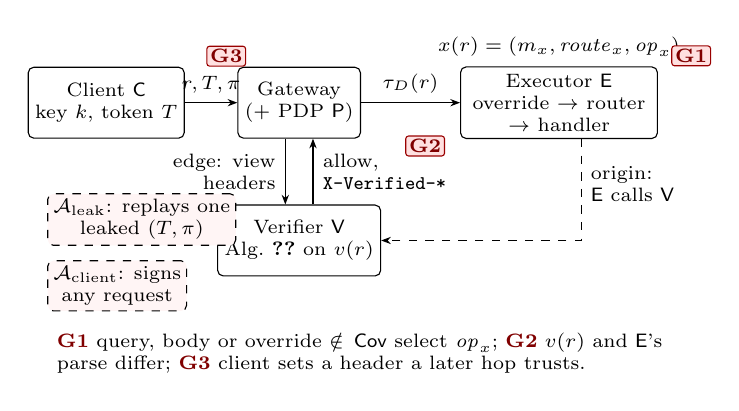
\begin{tikzpicture}[font=\scriptsize,
  box/.style={draw, rounded corners=2pt, align=center, inner sep=2.5pt, minimum height=0.9cm},
  adv/.style={draw, dashed, rounded corners=2pt, align=center, inner sep=2pt, fill=red!4},
  cls/.style={fill=red!12, draw=red!60!black, text=red!50!black, rounded corners=1pt,
     inner sep=1.2pt, font=\scriptsize\bfseries},
  >={Stealth[length=3.5pt]}]
\node[box] (C) at (0,0) {Client $\Cl$\\ key $k$, token $T$};
\node[box] (G) at (2.45,0) {Gateway\\ (+ PDP $\PDP$)};
\node[box, minimum width=2.5cm] (E) at (5.75,0) {Executor $\Exe$\\ override $\to$ router\\ $\to$ handler};
\node[box] (V) at (2.45,-1.75) {Verifier $\Ver$\\ Alg.~\ref{alg:verifier} on $\view(r)$};
\draw[->] (C) -- node[above]{$r,T,\pi$} (G);
\draw[->] (G) -- node[above]{$\tau_D(r)$} (E);
\draw[->] ([xshift=-5pt]G.south) -- node[left, align=right]{edge: view\\ headers} ([xshift=-5pt]V.north);
\draw[->] ([xshift=5pt]V.north) -- node[right, align=left]{allow,\\ \hdr{X-Verified-*}} ([xshift=5pt]G.south);
\draw[->, dashed] ([xshift=8pt]E.south) |- node[pos=0.22, right, align=left]{origin:\\ $\Exe$ calls $\Ver$} (V.east);
\node[above=0pt of E, font=\scriptsize] {$\exe(r)=(m_x,\mathit{route}_x,\op_x)$};
\node[cls, anchor=south] at ([xshift=12pt]E.north east) {G1};
\node[cls] at (4.05,-0.55) {G2};
\node[cls, anchor=south] at ([xshift=-4pt]G.north west) {G3};
\node[adv, anchor=north west] (AL) at (-0.75,-1.15) {$\Aleak$: replays one\\ leaked $(T,\pi)$};
\node[adv, anchor=north west] (AC) at (-0.75,-2.0) {$\Aclient$: signs\\ any request};
\node[align=left, anchor=north west, font=\scriptsize, text width=8.0cm] at (-0.75,-2.8) {%
\textbf{\textcolor{red!50!black}{G1}} query, body or override $\notin\Cov$ select $\op_x$;
\textbf{\textcolor{red!50!black}{G2}} $\view(r)$ and $\Exe$'s parse differ;
\textbf{\textcolor{red!50!black}{G3}} client sets a header a later hop trusts.};
\end{tikzpicture}
\Description{System and threat architecture: a client with key and token sends a request with a proof to a gateway that may host a policy decision point; the gateway forwards it to an executor made of override middleware, router and handler. Below the gateway, a verifier checks the proof against the view headers (edge placement); in origin placement the executor calls the verifier itself (dashed). Red tags mark where the three failure classes arise: G3 at the gateway boundary, G2 between the verifier's view and the executor's parse, G1 inside the executor. Two adversaries are shown: one who replays a leaked token and proof, and a legitimate client who signs any request.}
\caption{System and threat architecture. $\Ver$ checks $\pi$ against its view
$\view(r)$; $\Exe$ runs $\exe(r)$ on the request $\tau_D(r)$ the intermediaries
deliver. Edge placement reaches $\Ver$ through a gateway adapter; origin
placement calls it from $\Exe$ (dashed).}
\label{fig:arch}
\end{figure}

\subsection{System model}\label{sec:model:system}

A deployment $D$ consists of a client, a verifier, an optional policy decision
point, zero or more intermediaries and an executor (Figure~\ref{fig:arch}).
The client $\Cl$ holds a key $k$ and a token $T$ with $T.\jkt=\mathsf{th}(k)$,
the RFC~7638 thumbprint. For each request $r$ it signs a fresh proof
$\pi=(\htm,\htu,\ath,\jti,\iat)$. The \emph{canonical request} $r_\pi$ is the
request an honest client sends with $\pi$: method \htm, origin-form target the
path of \htu. Otherwise $r$ is an arbitrary byte string.

The verifier $\Ver$ maps the request it observes to a \emph{view}
$\view(r)=(m_v,u_v)$, taken from the gateway's own request line or from headers
such as \hdr{X-Forwarded-Uri} the gateway writes. $\Ver$ \emph{accepts} iff
Algorithm~\ref{alg:verifier} allows on that view; its comparison function
$\canon$ is a deployment parameter (RFC~9449 only recommends RFC~3986
normalisation). An optional PDP $\PDP$ maps the view and the subject to a
decision on a resource $\rho_\PDP(\view(r))$, e.g.\ a path-keyed policy.
The executor $\Exe$---router, override middleware and handler---receives
$\tau_D(r)$ and computes the \emph{executed operation}
$\exe(r)=(m_x,\mathit{route}_x,\op_x)$: the effective method after override,
the matched route with parameter assignment $\theta_x$, and the operation that
ran, including dispatch on the query or body. Two executions are the same
operation iff they agree on $\hat\exe(r)=(\op_x,\theta_x)$. Ground truth is
$\op(\pi)=\hat\exe(r_\pi)$ for $r_\pi$ sent directly to $\Exe$ without
intermediaries or verification.

\subsection{Binding soundness}\label{sec:model:soundness}

Let $\Acc_D(\pi)$ be the set of requests $r$ that the verifier accepts under
$\pi$ in $D$ and for which the executor runs an operation.

\begin{definition}[Binding soundness]\label{def:soundness}
$D$ is \emph{binding-sound} if, for every proof $\pi$ and all
$r,r'\in\Acc_D(\pi)$, $\hat\exe(r)=\hat\exe(r')$; it is \emph{binding-correct}
if moreover $\hat\exe(r)=\op(\pi)$ for every $r\in\Acc_D(\pi)$.
\end{definition}

\begin{definition}[Binding resolution]\label{def:resolution}
$\res_D(\pi)=\lvert\{\hat\exe(r) : r\in\Acc_D(\pi)\}\rvert$.
\end{definition}

$D$ is binding-sound iff $\res_D(\pi)\le 1$ for all $\pi$. In a functioning
deployment $r_\pi\in\Acc_D(\pi)$, so one accepted $r$ with
$\hat\exe(r)\neq\op(\pi)$ witnesses $\res_D(\pi)\ge 2$
(Figure~\ref{fig:views}). Our oracle searches for such witnesses; since it
observes finitely many requests, every reported resolution is a lower bound.
Binding soundness is weaker than message integrity: requests may differ in any
component provided the executed operation does not. It is the property
RFC~9449 implicitly relies on when it signs ``just enough''.

\begin{figure}[t]
\centering
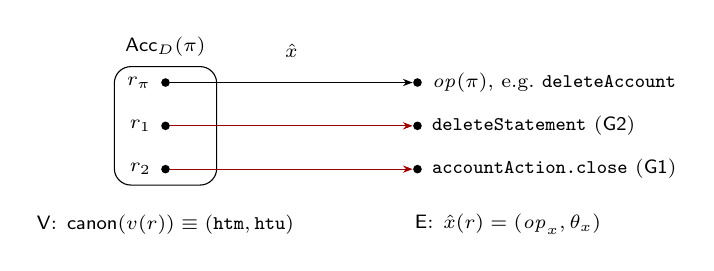
\begin{tikzpicture}[font=\scriptsize, >={Stealth[length=3.5pt]},
  dot/.style={circle, fill, inner sep=1.1pt},
  set/.style={draw, rounded corners=6pt, inner sep=4pt}]
\node[dot, label={[font=\scriptsize]left:$r_\pi$}] (r0) at (0,0.55) {};
\node[dot, label={[font=\scriptsize]left:$r_1$}] (r1) at (0,0) {};
\node[dot, label={[font=\scriptsize]left:$r_2$}] (r2) at (0,-0.55) {};
\node[set, fit=(r0)(r1)(r2), minimum width=1.3cm, label={[font=\scriptsize]above:$\Acc_D(\pi)$}] (A) {};
\node[font=\scriptsize, align=center] at (0,-1.25) {$\Ver$: $\canon(\view(r))\equiv(\htm,\htu)$};
\node[dot, label={[font=\scriptsize]right:$\op(\pi)$, e.g.\ \texttt{deleteAccount}}] (o0) at (3.2,0.55) {};
\node[dot, label={[font=\scriptsize]right:\texttt{deleteStatement} (\GB)}] (o1) at (3.2,0) {};
\node[dot, label={[font=\scriptsize]right:\texttt{accountAction.close} (\GA)}] (o2) at (3.2,-0.55) {};
\node[font=\scriptsize, align=center] at (4.35,-1.25) {$\Exe$: $\hat\exe(r)=(\op_x,\theta_x)$};
\draw[->] (r0) -- (o0); \draw[->, red!60!black] (r1) -- (o1); \draw[->, red!60!black] (r2) -- (o2);
\node[font=\scriptsize] at (1.6,0.95) {$\hat\exe$};
\end{tikzpicture}
\Description{Two columns of dots. On the left, the set of requests the verifier accepts under one proof: the canonical request and two mutated requests, all of which map to the same verifier view. On the right, executed operations. The canonical request maps to the proof's operation; the two mutated requests map to two other operations, one through an interpretation differential and one through query dispatch. Three distinct operations means binding resolution three.}
\caption{Binding soundness. All requests in $\Acc_D(\pi)$ look the same to
$\Ver$ (verifier view $\view(r)$), but $\Exe$ executes $\hat\exe(r)$; here
$\res_D(\pi)=3$, witnessed by a \GB and a \GA request.}
\label{fig:views}
\end{figure}

\begin{definition}[Authorization soundness]\label{def:authz}
A deployment with $\PDP$ is \emph{authorization-sound} if, whenever $\Ver$
accepts $r$ and $\PDP$ permits action $a$ on $\rho=\rho_\PDP(\view(r))$, the
executor acts only on $\rho$ with action $a$.
\end{definition}

Binding soundness concerns which operation a \emph{proof} selects;
authorization soundness concerns which resource a \emph{decision} selects. A
binding-soundness finding always involves a proof the adversary did not
create; an authorization-soundness finding involves none, because the client
signs exactly what it sends. We report the two separately and never add them.

\subsection{Failure classes}\label{sec:model:classes}

Let $\Cov=\{\text{method},\text{target URI without query},T\}$ be the covered
components and $\mathsf{in}_\Exe(r)=(m^\Exe,p^\Exe)$ the method and path as
the executor parses them, before override. A witness falls into one or more
classes.
\textbf{\GA, under-binding by design:} $\Exe$ reads the covered components as
$\Ver$ does, $(m^\Exe,\canon(p^\Exe))=(m_v,\canon(u_v))$, yet the operation
differs, so something outside $\Cov$ selected it: a dispatching query
parameter, a body field (GraphQL \texttt{operationName}, JSON-RPC), or a
method override (\hdr{X-HTTP-Method-Override}, \texttt{\_method}).
\textbf{\GB, interpretation differential:} $\Ver$ and $\Exe$ disagree on a
covered component, $(m^\Exe,\canon(p^\Exe))\neq(m_v,\canon(u_v))$---dot
segments, encoded separators, fragments, matrix parameters, duplicate slashes,
case, prefix rewrites.
\textbf{\GC, binding propagation:} a field that a downstream component treats
as the result of an upstream check (\hdr{X-Original-URI},
\hdr{X-Verified-Sub}, \hdr{Client-Cert}) is chosen by the client. \GC can make
$\view(r)$ client-controlled, turning acceptance into a \GB witness, or change
the subject the executor believes was verified.

\subsection{Adversaries}\label{sec:model:adversaries}

\paragraph{\Aleak, proof-leak adversary.} \Aleak obtains one valid
$(T,\pi)$, e.g.\ from logs or an intermediary's request log, and can send
arbitrary bytes to the public origin. It does not learn $k$, cannot mint or
alter proofs and cannot break TLS. Its goal is, within the \iat window, an
executed $\hat\exe(r)\neq\op(\pi)$. This matches attacker A5 of the FAPI~2.0
attacker model, which ``can also read requests sent to the resource
server''~\cite{fapiam2025}, though A5 sees them only after processing. Replay
state limits \Aleak but not everywhere: RFC~9449 notes that single-use \jti
checks may be infeasible without shared state and frames them ``in the
context of the target URI''. The harness sends only the mutated request per
fresh proof, with the replay cache on; this models deployments whose \jti
check does not reject it (the canonical request went to another replica, or
the cache is keyed per URI).

\paragraph{\Aclient, malicious legitimate client.} A registered client with
its own $k$ and $T$ and consent for resources $R$ (\texttt{alice} owns
\texttt{acc-alice-1}). It can mint any proof. Its goal is that $\Ver$ and
$\PDP$ approve $\rho\in R$ while $\Exe$ acts on $\rho'\notin R$
(Definition~\ref{def:authz}).

\paragraph{Excluded and scope.} We exclude network attackers (TLS is
assumed), malicious operators of gateway, verifier or executor, malware
holding $k$, a compromised authorization server~\cite{hosseyni2024csf}, and
denial of service. Harness traffic is cleartext HTTP/1.1 to
\texttt{http://api.bench.test}: view extraction, URI comparison, routing,
override and header forwarding happen after TLS termination, neither
adversary needs to break TLS, and certificate binding behind a proxy reduces
to the header that our \GC primitives test. HTTP/2 front ends appear only via
\texttt{h2c}. Hypotheses \Hyp{1}--\Hyp{5} and their falsifiers are in
Appendix~\ref{app:hyp}.

% sections/prevalence.tex -- Section 4: prevalence of under-binding (E1, E2). A1 moved to sections/ablation.tex (W25).
% Owner: W10 (wave 2). Every number is a macro from numbers.tex, whose comments name
% the source line in binding/prevalence/E1_results.md or E2_results.md (W8).
\section{Prevalence of Under-Binding (\GA)}\label{sec:prevalence}

\GA needs no bug: a proof bound to $(\htm,\htu)$ leaves the operation open
whenever the executor dispatches on something outside $\Cov$. Method
confusion and dispatch are known: Golinelli et al.\ show that applications
treat POST and GET interchangeably~\cite{p2:golinelli2026post}, and
CVE-2026-37236 shows an \hdr{X-HTTP-Method-Override} bypassing upstream method
ACLs~\cite{grpcgw2026cve37236}. Our contribution is to measure how often a
proof-bound request is exposed: how often API descriptions put several
operations behind one (method, path) key (\Exp{1}), and how often method
override---which survives a proof-bound \htm because it is resolved after
verification---is reachable (\Exp{2}).

\subsection{API descriptions (\Exp{1})}\label{sec:prev:e1}

\paragraph{Method.} The verifier's view is the key $K = (\textit{method},
\textit{path})$. A key is \emph{collided} if the description maps it to two or
more operations selected by a query parameter, a header or a body field. We
analyse the APIs.guru OpenAPI directory (one pinned commit, cloned 2026-11-22):
\NumSpecFiles{} spec files, of which \NumSpecFilesParsed{} parsed
(\NumSpecFilesFailed{} YAML errors excluded). The unit is one preferred spec per
API, giving \NumSpecs{} APIs with \NumOps{} operations, \NumStateChangingOps{}
of them state-changing (POST, PUT, PATCH or DELETE). Five detectors flag
collisions: a query or fragment inside the path key (M1), a dispatcher-named
parameter with an enum of at least two values (M2), header dispatch such as
\hdr{X-Amz-Target} (M3), a discriminated body union or dispatcher-named body
field (M4), and JSON-RPC or GraphQL single endpoints (M5). Only their strong
tiers are counted.

\paragraph{Validation.} One author judged a seeded, detector-stratified sample of
\NumValidationSample{} flagged operations against the spec text (unclear counts as false positive). Precision is
\PrecMOne{} for M1 (\NumMOneTP/\NumMOneSample), \PrecMTwo{} for M2, \PrecMFour{} for M4 and
\PrecMFive{} for M5 (\NumMFiveFlags{} flags). Weighted by stratum it is \PrecWeighted{}
overall, but only \PrecNonMOneWeighted{} outside M1. We therefore also report a
hand-confirmed lower bound.

\begin{table}[t]
\caption{\Exp{1}: state-changing operations on a collided (method, path) key.
Raw detector counts, strong tier; 95\% Wilson intervals in brackets.}
\label{tab:e1}
\small
\begin{tabular}{@{}l r r r@{}}
\toprule
Subset & APIs & APIs collided & State ops collided \\
\midrule
All & \NumSpecs & \NumApisCollided{} (\PctApisCollided) & \NumStateOpsCollided{} (\PctUnderBound) \\
Excl.\ AWS & \NumSpecsNonAWS & \NumApisCollidedNonAWS{} (\PctApisCollidedNonAWS) & \NumStateOpsCollidedNonAWS{} (\PctUnderBoundNonAWS) \\
Excl.\ hyperscalers & \NumSpecsNonHyper & \NumApisCollidedNonHyper{} (\PctApisCollidedNonHyper) & \NumStateOpsCollidedNonHyper{} (\PctUnderBoundNonHyper) \\
Finance & \NumSpecsFinance & \NumApisCollidedFinance{} (\PctApisCollidedFinance) & \NumStateOpsCollidedFinance{} (\PctUnderBoundFinance) \\
\bottomrule
\end{tabular}
\end{table}

\paragraph{Results.} Table~\ref{tab:e1} gives the raw counts.
\PctUnderBound{} \CIUnderBound{} of the \NumStateChangingOps{} state-changing
operations in the corpus sit on a collided key. Nearly all of this comes from
AWS's query and RPC protocols: \NumMOneOpsAWS{} of the \NumMOneOps{} M1 flags
are AWS operations, and EC2 alone puts \NumEcTwoOpsPerKey{} operations on each of
\texttt{POST /} and \texttt{GET /}. AWS itself is not exposed, because SigV4
signs the query and \hdr{X-Amz-Target}; it shows how common the protocol pattern
is. Outside AWS, \PctApisCollidedNonAWS{} \CIApisCollidedNonAWS{} of APIs are
flagged, and the hand-confirmed figure is \NumConfirmedApisNonAWS{} of
\NumSpecsNonAWS{} (\PctConfirmedApisNonAWS); the true share lies between the
two, nearer the lower end given the M2 and M4 precision. A census of all
\NumFinanceFlagged{} finance flags confirmed \NumFinanceTP{}, in
\NumFinanceApisTP{} of \NumSpecsFinance{} finance APIs. The confirmed
collisions select high-impact commands: Stripe's usage records
(\texttt{action=increment|set}), Zuora refunds (\texttt{settle|reject}),
Zoom's \texttt{DELETE /users/\{id\}?action=disassociate|delete}, and openSUSE's \texttt{POST /person/\{login\}}, whose \texttt{cmd} parameter selects \texttt{change\_password}, \texttt{lock} or \texttt{delete}. Only
\NumApisDocOverride{} APIs (\PctApisDocOverride, all Amadeus) document a method
override, which is a framework property that descriptions rarely state
(\S\ref{sec:prev:e2}). Using every spec version instead of one per API changes
the headline share to \PctUnderBoundAllFiles{} (\PctUnderBoundAllFilesNonAWS{}
excluding AWS).

\paragraph{Standards that under-bind by construction.} Two specifications
outside the corpus make \GA the normal case. In HL7 FHIR, conditional
update and delete select their targets by query, and a \texttt{POST [base]}
transaction Bundle carries every CRUD interaction in its body; the public HAPI
FHIR R4 server declares conditional update, create and delete for all
\NumFhirTypesConditional{} resource types. The Model Context Protocol sends every
tool call as a POST to one endpoint and selects the operation by the JSON-RPC
body. Its 2026 revision mirrors the method and tool name into headers and
requires servers to reject mismatches, citing exactly the split-view risk of
\GB; DPoP does not occur in the MCP specification files we pinned. A proof
for either protocol names an endpoint, not an operation.

\subsection{Framework method override (\Exp{2})}\label{sec:prev:e2}

\paragraph{Method.} For \NumTargetFrameworks{} target frameworks (and Symfony,
Jersey, Hono and gorilla/handlers for comparison) we read the override code at a
pinned release tag and the vendor documentation. All \NumPinnedSourcesVerified{}
pinned source files were re-fetched and compared byte for byte, and all
\NumDocChecks{} documentation claims were checked against the fetched pages. To
estimate how often projects enable an opt-in mechanism, we use GitHub code
search counts; these are engine estimates over files, so we report them only as
orders of magnitude.

\paragraph{Results.} Override is reachable in the default configuration of
\NumOverrideFrameworks{} of the \NumTargetFrameworks{} frameworks. Rails keeps
\texttt{Rack::MethodOverride} unless an app is API-only, and Laravel enables
Symfony's override on every request, including the
\hdr{X-HTTP-METHOD-OVERRIDE} header for any POST. It is opt-in in
\NumOptInFrameworks{} (Spring Boot since 2.2, ASP.NET Core, Express through the
\texttt{method-override} package) and absent in \NumNoOverrideFrameworks{}
(FastAPI/Starlette, Django, Go \texttt{net/http} and chi, where the only method
change is HEAD to GET). Every built-in mechanism rewrites only POST, so the
transition is always \emph{a proof for POST executing PUT, PATCH or DELETE}.
The variant that reads \texttt{\_method} from the \emph{query} is the worst
case for DPoP, since \htu omits the query: it is reachable in Spring MVC,
Express with \texttt{methodOverride('\_method')}, gorilla/handlers,
Laravel/Symfony and Jersey. ASP.NET Core accepts any override value, with no
allowlist.

Where override is opt-in, roughly 1--2\% of projects turn it on (Spring
\PctEnableSpring{}, Express \PctEnableExpress{} of \texttt{package.json} files,
\PctEnableExpressNpm{} by npm downloads, gorilla \PctEnableGorilla{}); ASP.NET
Core is lower (\PctEnableAspnet{}). Where it is on by default it stays on: only
\PctRailsApiOnly{} of Rails application files declare API-only mode, so about
\PctRailsOverrideOn{} keep the middleware, and Laravel has no switch. Among
Express projects that use the package, \PctExpressQueryGetter{} of the two
common call forms choose the query getter.

\paragraph{Limitations.} The corpus over-represents hyperscalers and
under-represents GraphQL, gRPC and private APIs; recall is unmeasured, so
counts are lower bounds; one author judged the sample. A collision means a
proof bound to $K$ would be ambiguous, not that the API accepts DPoP.
Code-search ratios are engine estimates. Override is exploitable only if a
POST route shares its path with a state-changing route and the verifier sits
in front of the override, which the harness tests (\S\ref{sec:results}).

% sections/harness.tex -- Section 5: harness and methodology. Written from the component READMEs in
% binding/harness/* and executors/*/CONFORMANCE.md (W10); Alg. 2 transcribes
% ../harness/oracle/oracle_spec.md §2-§4 (W25). Results are in sections/results.tex.
\section{Harness and Methodology}\label{sec:harness}

The prevalence study shows where a proof \emph{could} be ambiguous. The
harness tests whether real gateways, a correct verifier and real frameworks
let one proof select more than one operation. All components are containers
on one host; every request carries \hdr{Host: api.bench.test}.

\paragraph{Tokens and verifier.} A test authorization server issues ES256
access tokens bound to one of two clients, each owning one account. For every
case the minter signs a fresh proof for the canonical $(\htm,\htu)$ of the
case's \emph{base} operation; the request is then mutated, and the proof's
\jti is the correlation key in every log. One reference verifier
(Algorithm~\ref{alg:verifier}) serves every gateway through three adapters:
\hdr{X-Forwarded-*} headers (Traefik ForwardAuth, APISIX \texttt{forward-auth}),
\hdr{X-Original-*} headers (NGINX \texttt{auth\_request}, Kong, HAProxy, and
executors in origin placement), or the Envoy \texttt{ext\_authz} check request.
The \htu comparison is exact, RFC~3986 normalisation (default), or a
\texttt{strict} mode that rejects dot segments, encoded separators and empty
segments. A single verifier means a witness is attributable to the deployment,
not to a verifier bug.

\paragraph{Gateways and executors.} \NumGateways{} gateways are pinned by tag
and digest: Envoy 1.39.6, Traefik 3.7.19, NGINX 1.30.7, Kong OSS 3.9.5 (a
pre-function, since OSS ships no forward-auth plugin), APISIX 3.21.0 and
HAProxy 3.2.27 (a Lua action). Each has \NumGatewayProfiles{} profiles:
\emph{default} (vendor defaults plus routing and the verifier call),
\emph{recommended} (vendor-documented normalisation and header hygiene, each
with its documentation link) and \emph{strict} (strictest native options plus
a harness-defined deny rule; a ceiling, not a vendor setting).
\NumFrameworks{} frameworks implement one bench API (Table~\ref{tab:exec} in
Appendix~\ref{app:hyp}): \NumBenchOps{} canonical operations under
\texttt{/api}, logged as \NumBenchOpIds{} operation identifiers because an
action endpoint dispatches on the query parameter \texttt{op} and a GraphQL
endpoint on \texttt{operationName}. \texttt{OVERRIDE=on} enables the
framework's own or de-facto standard override middleware, never custom code;
for Rails and Laravel this is the stock configuration. In origin placement the
executor calls the verifier with the raw request line
(\texttt{origin-raw}) or with the effective method and matched route
(\texttt{origin-routed}, defence D-A). Executors log the raw and effective
method, raw target, matched template, path parameters and trust headers.

\paragraph{Mutations and transport.} The catalogue has \NumPrimitives{}
primitives (\NumPrimitivesGOne{} \GA, \NumPrimitivesGTwo{} \GB,
\NumPrimitivesGThree{} \GC), each citing the paper, advisory or RFC it comes
from (Appendix~\ref{app:primitives}). \GA primitives add override headers or
\texttt{\_method}, switch \texttt{op}, or swap \texttt{operationName}; \GB
primitives cover dot segments, encoded and duplicate slashes, matrix
parameters, case, absolute-form targets, backslashes, fragments, NUL and
overlong encodings and prefix rewrites; \GC primitives inject or alias view,
identity and certificate headers, including a forged \hdr{X-Verified-View}.
Depth-1 cases apply every primitive to every compatible base operation. The
runner writes exact bytes to a TCP socket, since any HTTP library would
normalise the mutation away.

\begin{algorithm}[t]
\caption{Binding oracle for one case (base operation $b$, placement $P$),
after \texttt{oracle\_spec.md}.}\label{alg:oracle}
\KwIn{ground truth $\op(\pi)=(b,\theta^*)$ from $r_\pi$ sent directly to $\Exe$ with verification off; logs $R, \mathit{VS}, \mathit{XS}$ joined on $\pi.\jti$}
\KwOut{hit (with deviation kinds) or no hit}
\lIf{$\op(\pi).\op\neq b$ or status $\ge 400$}{\Return excluded (\emph{nonconformant})}
\ForEach{executor record $x\in\mathit{XS}$}{
  $A_e\gets\exists v\in\mathit{VS}: v.\mathsf{dec}=\mathsf{allow}$;\quad $A_o\gets\neg x.\mathsf{denied}\wedge$ origin call allowed\;
  $A\gets A_e$ (edge), $A_o$ (origin), $A_e\wedge A_o$ (both)\Cmt*[f]{accepted}\;
  $B\gets x.\op\notin\{b,\textsf{NOT\_FOUND}\}\ \vee\ (x.\op=b \wedge x.\theta\neq\theta^*)$\Cmt*[f]{dispatch/route/method, or resource}\;
  \lIf{$A\wedge B\wedge x.\mathsf{status}<400$}{\Return hit, kinds $\subseteq\{$method, route, dispatch, resource$\}$}
}
\Return no hit\Cmt*[f]{executed without a verifier record: class B0, never a hit}
\BlankLine
\textbf{Resolution} for $(D,b)$: $\widehat{\res}=\lvert\{\op(\pi)\}\cup\{\hat\exe(x): A\wedge x.\mathsf{status}<400\wedge x.\op\neq\textsf{NOT\_FOUND}\}\rvert\le\res_D(\pi)$\;
\end{algorithm}

\paragraph{Oracle.} Algorithm~\ref{alg:oracle} is the definition turned into a
test. Ground truth is measured, not assumed; an executor that disagrees with
the bench API is marked non-conformant and excluded (none was). A hit needs an
accepted request, a different executed operation or resource, and a status
below 400. Spoofed headers that reach the executor without changing the
operation are reported by a separate \GC \emph{propagation} predicate; an
executed request with no verifier record is a verifier bypass (B0). Neither
counts as a hit. Hits are deduplicated by a root-cause signature (topology
factors, minimal primitive set from delta debugging over primitives and bytes,
class, deviation kind) and rerun three times, each with a fresh proof against a
freshly started topology; only hits confirmed 3/3 are counted. The oracle is a
pure function of the logs.

\paragraph{Validation.} The verifier passes \NumVerifierTests{} tests,
including one negative test per item of the OpenID conformance suite's DPoP
list. All \NumFrameworks{} executors pass a shared conformance suite
(\NumConformanceCases{} cases, every configuration). All
\NumSmokePass{}/\NumSmokeRuns{} gateway smoke runs reached the right adapter,
view and operation. In every topology the honest request must be accepted and
execute $\op(\pi)$, or the topology is excluded.

\paragraph{Matrix.} The design space has \NumMatrixTopologies{} topologies
(gateway $\times$ profile $\times$ placement $\times$ framework $\times$
override). We ran four slices under \Aleak and one under \Aclient
(Table~\ref{tab:campaign}). The \emph{edge} slice covers every gateway and
framework, the default and recommended profiles and both override settings
(\NumTopoVOneEdge{} topologies, \NumCasesVOne{} cases each). The
\emph{placement} slice (\Abl{3}) moves the verifier into the executor. The
\emph{route} slice adds \NumNewRoutes{} routes behind a switch: a POST sharing
its path with GET/PUT/DELETE, a nested same-method route, a deeper nested
DELETE and a catch-all. All runs used real components, one topology at a time
per worker, on one 16\,GB, 10-core host.

\begin{table}[t]
\caption{Campaign. Requests are raw-socket cases; every hit was re-run three
times on a freshly started topology.}
\label{tab:campaign}
\scriptsize
\setlength{\tabcolsep}{3pt}
\begin{tabular}{@{}l l r r r r@{}}
\toprule
Slice & Factors & Topol. & Requests & Hits & \GB \\
\midrule
Edge & NGINX, Traefik, Envoy $\times$ 4 fw & \NumTopoKill & \NumCasesKill & \NumHitsKill & \NumGTwoKill \\
Edge & Kong, APISIX, HAProxy $\times$ 8 fw & \NumTopoExtGw & \NumCasesExtGw & \NumHitsExtGw & \NumGTwoExtGw \\
Edge + \Abl{3} & 3 gw $\times$ 4 fw; origin/both $\times$ 8 fw & \NumTopoExtFw & \NumCasesExtFw & \NumHitsExtFw & \NumGTwoExtFw \\
Routes (v2) & NGINX, Envoy $\times$ 8 fw & \NumTopoExtRoutes & \NumCasesExtRoutes & \NumHitsExtRoutes & \NumGTwoExtRoutes \\
\midrule
\Aleak total & & \NumTopologies & \NumCases & \NumHits & \NumHitsGTwo \\
\Aclient{} + PDP & 6 gw $\times$ 6 fw $\times$ 2 policies & \NumEFourTopologies & \NumEFourCases & \NumEFourViolations$^{a}$ & -- \\
\bottomrule
\end{tabular}\\[1pt]
{\scriptsize $^{a}$authorization-soundness violations, not binding hits (\S\ref{sec:results:e4}).}
\end{table}

% sections/results.tex -- Section 6: security testing results (W25, from the W19 text).
% Sources: experiments/{kill/G1_REPORT,ext-gw,ext-fw,ext-routes,e4}/REPORT.md, GATE_DECISION.md,
% disclosure/TRIAGE.md, lit/pass2/NOVELTY_UPDATE.md (C3, C4: APISIX reclassified, E4 = reproduction).
% Every number is a numbers.tex macro naming its source.
\section{Results: Binding Soundness in Practice}\label{sec:results}

\paragraph{Totals.} The \NumTopologies{} \Aleak topologies received
\NumCases{} requests with \NumTransportErrors{} transport errors, neither on a
hit case. The oracle reported \NumHits{} hits (\NumSOneHits{} S1,
\NumSTwoHits{} S2, none S3); \NumVulnTopologies{} topologies have
$\widehat{\res}>1$ for some base operation. Every hit reproduced 3/3 on a
freshly started topology with a fresh proof (\NumConfirmedHits{} rerun
directly; for Kong, APISIX and HAProxy only the default profile was rerun,
because the recommended-profile hits were byte-identical). We saw
\NumFlaky{} flaky hits and \NumBZero{} verifier bypasses.

\paragraph{By class.} By mechanism, \NumHitsGOne{} hits are \GA and
\NumHitsGTwo{} \GB, in \NumGTwoTopologies{} topologies; there are
\NumHitsGThree{} \GC binding hits. (By primitive label there are
\NumHitsGOneOracle{} and \NumHitsGTwoOracle{}: delta debugging moved
\NumHitsRCSeven{} \GB-labelled hits to \GA, because a \texttt{\#} landing in
the \emph{query} minimises to one extra byte in the unbound \texttt{op}.)
Figure~\ref{fig:heatmap} shows the edge slice: \GA is constant down every
column---the gateway never changes it, and default and recommended profiles
gave identical hits in all \NumTopoVOneEdge{} edge topologies---while \GB is
confined to three gateways and depends on the backend.
Figure~\ref{fig:class} splits hits by campaign and primitive family,
Figure~\ref{fig:resolution} gives resolution, and Table~\ref{tab:rc} lists the
root causes.

\begin{figure*}[t]
\centering
\figpdf{\textwidth}{4.3cm}{fig_hits_heatmap.pdf}
\Description{Two heatmaps with gateways as rows and frameworks as columns. The G1 panel has similar values in every cell, the same down each column. The G2 panel is zero except for NGINX and Kong with FastAPI, go-chi and Laravel, and APISIX with Express, go-chi, ASP.NET and Rails.}
\caption{Binding hits per gateway $\times$ framework (\Aleak, edge
placement, v1 routes; each cell sums four topologies: two profiles, override
off/on). (a)~\GA under-binding is present in every cell; (b)~\GB
differentials are confined to NGINX/Kong $\times$ FastAPI/chi/Laravel
(\texttt{\#} in the path) and APISIX $\times$ Express/chi/ASP.NET/Rails
(encoded slash).}
\label{fig:heatmap}
\end{figure*}

\begin{figure}[t]
\centering
\figpdf{\linewidth}{4.6cm}{fig_resolution.pdf}
\Description{Bar chart on a log scale of how many topology and base-operation pairs have binding resolution one to six, split into the v1 and v2 route spaces. Most pairs have resolution one; resolution two and three are common; four to six occur only rarely, five and six only with v2 routes.}
\caption{Distribution of binding resolution $\widehat{\res}$, the number of
distinct operations one valid proof reaches, over all \NumResPairs{}
(topology, base operation) pairs: 1 for \NumResOne{}, 2 for \NumResTwo{}, 3
for \NumResThree{}, 4 for \NumResFour{}, 5 for \NumResFive{}, 6 for
\NumResSix{} (5 and 6 only with v2 routes). $\widehat{\res}>1$ violates
binding soundness.}
\label{fig:resolution}
\end{figure}

\begin{figure*}[t]
\centering
\figpdf{\textwidth}{4.3cm}{fig_class.pdf}
\Description{Left: stacked bars of binding hits per campaign by mechanism class; G1 dominates every campaign, G2 is a minority, G3 is zero. Right: horizontal bars of hits per primitive family across all campaigns, led by query dispatch, body _method and JSON-body dispatch, then fragment, header override, content-type relabel, encoded slash, dot segment and query _method.}
\caption{(a)~Binding hits per campaign by class (by mechanism): \GA dominates,
\GB contributes \NumHitsGTwo{} of \NumHits{}, and no \GC binding hit was
observed. (b)~Hits per primitive family across all campaigns; \GA primitives
drive \AblFourGOneShare{} of hits.}
\label{fig:class}
\end{figure*}

\begin{table*}[t]
\caption{Root causes, one row per independent mechanism (resolving component
$\times$ differential); current releases, default profile, unchanged by the
recommended one. Witnesses are ddmin outputs; \texttt{.../a1} is
\texttt{/api/v1/accounts/acc-alice-1}. ``Prior'' names the known family each
row belongs to. $^{\dagger}$Mechanism unconfirmed (see text).}
\label{tab:rc}
\scriptsize
\setlength{\tabcolsep}{2.6pt}
\begin{tabular}{@{}l l p{4.7cm} p{3.4cm} r p{3.2cm} p{2.6cm}@{}}
\toprule
ID & Cl. & Mechanism (verifier or PDP view vs.\ executor) & Where & Hits & Minimal witness & Prior \\
\midrule
\multicolumn{7}{@{}l}{\emph{Binding soundness, \Aleak: one leaked proof, the executor runs an operation other than $\op(\pi)$}} \\
B1 & \GB & verifier drops \texttt{\#\ldots} as fragment; gateway forwards it raw; server keeps it in the path & NGINX, Kong $\times$ uvicorn/h11, Go \texttt{net/http}, FrankenPHP & \NumHitsFragAll & \texttt{DELETE .../a1\#/statements/s-evil} $\to$ \texttt{deleteStatement} & CVE-2021-39156~\cite{p2:istio2021_008}; \cite{w2:uvicorn1222} \\
B2$^{\dagger}$ & \GB & verifier view lacks \texttt{\%2f}; upstream receives it raw & APISIX $\times$ ASP.NET, Express, chi, Rails & \NumHitsApisixPct & \texttt{DELETE /api/v1/accounts/}\allowbreak\texttt{\%2facc-alice-1} & CVE-2026-124680 post-fix~\cite{p2:apisix2026_124680} \\
B3 & \GB & verifier removes \texttt{./}; catch-all keeps it (\texttt{..} denied) & NGINX, Envoy $\times$ \NumFwXThree{} fw (v2) & \NumHitsXThree & \texttt{GET /api/v1/files/}\allowbreak\texttt{reports/./logo.png} & CVE-2026-40912~\cite{traefik2026cve40912} \\
G1-d & \GA & query \texttt{op}, JSON \texttt{operationName}, Content-Type not covered & all gw $\times$ all fw & -- & \texttt{POST .../a1/actions?op=close} & RFC~9449 \S4.2 \\
G1-o & \GA & override rewrites the method after the check & all fw with override; default: Rails, Laravel & -- & \texttt{POST .../a1}, body \texttt{\_method=DELETE} & \cite{p2:golinelli2026post,grpcgw2026cve37236} \\
\midrule
\multicolumn{7}{@{}l}{\emph{Authorization soundness, \Aclient: own valid proof passes; a path policy is split from the executor (reproduction of known patterns)}} \\
RC1 & \GB & Kestrel resolves \texttt{/../} before routing & ASP.NET behind NGINX, Envoy, HAProxy & \EFourRCOneViol & \texttt{GET .../a1/../acc-bob-1} & \cite{p2:zhang2025uabscan} \\
RC2 & \GB & Kong authorizes the raw target, proxies the normalised path & Kong $\times$ all 6 fw & \EFourRCTwoViol & as RC1 & \cite{p2:xvnpw2021kong,w2:kongcve27306} \\
RC3/4 & \GB & case-insensitive routing & ASP.NET / Express & \EFourRCThreeViol/\EFourRCFourViol & \texttt{GET /api/v1/ADMIN/users} & \cite{p2:zhang2025uabscan} \\
RC5 & \GB & matrix parameters stripped before matching & Spring & \EFourRCFiveViol & \texttt{GET /api/v1/}\allowbreak\texttt{accounts;/acc-bob-1} & \cite{p2:tsai2018breaking,p2:zhang2025uabscan} \\
RC6/7 & \GB & \texttt{//} collapsed (Rails) / as RC2 for \texttt{//} (Kong) & Rails; Kong $\times$ 4 fw & \EFourRCSixViol/\EFourRCSevenViol & \texttt{GET /api/v1/}\allowbreak\texttt{/accounts/acc-bob-1} & \cite{p2:zhang2025uabscan,p2:xvnpw2021kong} \\
\midrule
\multicolumn{7}{@{}l}{\emph{Propagation (\GC), conditional on a backend that trusts the header}} \\
P1 & \GC & client \hdr{Client-Cert}, \hdr{X-Forwarded-Client-Cert} reach the executor & all gw (Envoy strips XFCC) & 0 & -- & RFC~9440 \\
P2 & \GC & client \hdr{X-Verified-View} (D-B) reaches the executor & Envoy, Kong, HAProxy & 0 & -- & -- \\
\bottomrule
\end{tabular}
\end{table*}

\subsection{Interpretation differentials (\GB) under \Aleak}

Every differential we observe belongs to a known CVE family; prior work and
advisories treat them as bypasses of path-based policies. What changes here is
that the check is cryptographic and passes, and the executed operation differs.

\emph{B1, fragment in the path.} RFC~9112 forbids \texttt{\#} in an
origin-form target, yet NGINX and Kong forward it. The verifier parses it as a
fragment, which RFC~9449 excludes from the comparison, and accepts; uvicorn/h11,
Go \texttt{net/http} and FrankenPHP keep it in the path (Traefik and Envoy
reject it; Tomcat and Kestrel answer 400). In the v1 route space this only
suffixes the last parameter (\NumHitsFragPath{} hits, S1 by the oracle rule
but low practical impact). With a nested route it changes the operation: a
leaked \texttt{deleteAccount} proof runs \texttt{deleteStatement} and a leaked
\texttt{getAccount} proof runs \texttt{getStatements} (\NumHitsXOne{} hits,
default profile, override off); the attacker cannot choose the target
identifier. The lenient \texttt{\#} handling is known~\cite{w2:uvicorn1222};
notably, the RFC~9449 verifier's own normalisation---discarding the
fragment---is the remedy Istio adopted for CVE-2021-39156~\cite{p2:istio2021_008};
applied only to the verifier's view while the gateway forwards the raw target,
it creates the split rather than closing it.

\emph{B2, encoded slash behind APISIX (a variant, not a new class).} For
\texttt{DELETE /api/v1/accounts/\%2facc-alice-1} the verifier logged and
allowed the view \texttt{/api/v1/accounts/acc-alice-1}, while the executor
received the raw \texttt{\%2f}; Express and Rails decode it into another
identifier and ASP.NET and chi keep it literally (\NumHitsApisixPct{} hits).
The upstream half is deliberate: the fix for CVE-2026-124680 in APISIX
(PR~\#14035, in our 3.21.0 pin) forwards the original request line when
nginx did no more than percent-decode, precisely so that \texttt{\%2F}
survives~\cite{p2:apisix2026_124680}. B2 is therefore a consequence of that
accepted residual in a family with two 2026
CVEs~\cite{p2:apisix2026_94269,p2:apisix2026_124680}. One caveat remains:
APISIX's published \texttt{forward-auth} plugin sets \hdr{X-Forwarded-Uri}
from \texttt{ctx.var.request\_uri}, which should be raw, and this conflicts
with the decoded view our verifier logged; we have not reconciled the two, so
the mechanism of the verifier-side half is unconfirmed. Kong sends the raw
target and the verifier denies it; HAProxy uses one parsed URI for check and
upstream and has no \GB hit.

\emph{B3, dot segment.} RFC~3986 normalisation removes \texttt{./}; the v1
routers then return 404 (\NumLatentDot{} accepted-then-404 cases), but a
catch-all executes the raw path. Only the no-op segment passes, since the
verifier denies every traversal; we list B3 for completeness.

\paragraph{Resolution.} The action and GraphQL bases have $\widehat{\res}=3$ in
every v1 topology (\GA). The v1 maximum is \MaxResolutionVOne{}, where
FastAPI's any-method override meets B1; with v2 routes it is
\MaxResolution{} for the get, update and delete account operations. \texttt{adminDeleteUser}, \texttt{getAccountV2} and
\texttt{publicFile} have no query, body or override lever; their resolution
exceeds 1 only behind NGINX, Kong (B1) and APISIX (B2), which isolates the
contribution of \GB.

\subsection{Under-binding (\GA) and propagation (\GC)}

Query and body dispatch change the operation behind all \NumGateways{}
gateways and \NumFrameworks{} frameworks: this is the scope RFC~9449 states,
measured. Method override is the framework-level lever. In the v1 routes it
reached another operation only through FastAPI's Flask-style middleware, which
honours the header on any method; the standard middlewares override only POST
and no v1 POST shares a path. The v2 route \texttt{POST /accounts/\{id\}}
closes this gap: a leaked POST proof runs \texttt{updateAccount} or
\texttt{deleteAccount} in all \NumFrameworks{} frameworks with override on
(\NumHitsOverrideVTwo{} hits), which is the default configuration in Rails
(non-API) and Laravel (\S\ref{sec:prev:e2}).
No \GC primitive changed the executed operation: gateways overwrite
\hdr{X-Verified-Sub}/\hdr{-Jkt} from the verifier's response, and case and
underscore variants did not pass. Certificate headers pass every gateway
except Envoy (XFCC), and a forged \hdr{X-Verified-View} reaches the executor
behind Envoy (when no verifier header is set), Kong and HAProxy; both matter
only to a backend that trusts the header (P1, P2).

\paragraph{Placement (\Abl{3}).} Verifying at the executor on the raw request
removes no \GA hit (behind Envoy, \NumHitsEnvoyOrigin{} hits remain across
\NumFrameworks{} frameworks) and keeps B1 behind NGINX
(\NumHitsNginxOriginFixed{} hits), since the executor's verifier call strips
the fragment before the handler binds it. Two apparent zeros were artefacts:
NGINX's default \texttt{proxy\_pass} rewrites \hdr{Host}, failing every origin
check including the honest one (we fixed \hdr{Host} and re-ran), and
\emph{both} placement presents one single-use \jti twice, so the origin call
fails as a replay (\NumJtiReplayEnvoyBoth{} of \NumCasesVOne{} cases behind
Envoy). Re-checking the same proof at the origin is no defence; the origin
must check the \emph{routed} view (\S\ref{sec:defence}).

\subsection{Authorization soundness under \Aclient: a reproduction}\label{sec:results:e4}

Path-policy bypasses caused by gateway/backend normalisation differences are
well documented, from practitioner research on external-authorisation
plugins~\cite{p2:xvnpw2021kong,p2:xvnpw2022ingress,p2:tsai2018breaking} to
systematic studies of routing/authentication inconsistencies in Java
applications~\cite{p2:zhang2025uabscan} and nginx
configurations~\cite{p2:sadeghi2026nginxbuster}, and continue to produce CVEs
in current gateways~\cite{p2:traefik2026_88009,p2:apisix2026_124680,p2:envoy2026_73551}.
We include them not as new findings but to show that sender-constraining is
orthogonal to them: a client holding a valid, correctly verified DPoP proof
can still reach operations its gateway policy denies. NginxBuster is
concurrent work on the nginx \texttt{auth\_request} placement we use.

\paragraph{Setup and results.} A PDP runs the reference verifier and then
matches the \emph{same view} against a path policy: a default-deny allow-list
of \texttt{alice}'s resources, or a default-allow block-list of admin and
foreign-account regexes. \texttt{alice} mints a valid proof for every mutated
request, so only the policy stands in the way. Over \NumEFourVectors{} vectors
we observed \NumEFourViolations{} violations (\NumEFourAdmin{} admin,
\NumEFourBob{} cross-tenant) in \NumEFourVulnTopologies{} of
\NumEFourTopologies{} topologies, in \NumEFourClasses{} classes
(Table~\ref{tab:rc}); one topology per class was rerun three times and every
vector reproduced, and controls behaved. As in prior work, the dot-segment
classes are the strongest: Kestrel (RC1) and Kong's raw-\texttt{\$request\_uri}
authorization (RC2, the configuration and payload of xvnpw
2021~\cite{p2:xvnpw2021kong}) defeat even the strict allow-list. Traefik,
APISIX and Envoy's recommended profile normalise before the check
(\NumEFourHtuMismatch{} \htu denials). Authorizing on the routing view helps:
NGINX's native \texttt{location} ACL closed the dot-segment classes, while
Envoy RBAC was bypassed by \NumNativeEnvoyRaw{} vectors with the default
\texttt{normalize\_path: false}. The matrix covers \NumEFourTopologies{} of
\NumEFourCells{} cells and omitted absolute-form targets and
\hdr{X-Original-URL}, so class counts are lower bounds.

% sections/defence.tex -- Section 6: defences D-A and D-B (E7/E8, A2).
% Results produced by W17 (binding/experiments/defence/REPORT.md); numbers via numbers.tex macros.
\section{Restoring Binding Soundness}\label{sec:defence}

The results of \S\ref{sec:harness} rule out two easy fixes. Re-verifying
the same proof at the origin keeps every \GA hit and the \texttt{\#}
differential (\Abl{3}), and RFC~3986 normalisation in front of a path
policy closes only the dot-segment classes. We therefore evaluate two
defences that bind the check to the \emph{executor's} view.
\emph{D-A} (\texttt{origin-routed}): the executor calls the verifier with
the effective method after override resolution and the canonical path of
the route it actually matched. \emph{D-B} (view-binding MAC): the verifier
returns
$\hdr{X-Verified-View} = \mathrm{HMAC}_K(\jti \| m_v \| \canon(u_v) \| \jkt)$,
and the executor recomputes it from its routed view and rejects any mismatch.
For D-B, the gateway must strip a client-supplied \hdr{X-Verified-View}, which
Envoy, Kong and HAProxy do not do by default (P2 in Table~\ref{tab:rc}).

\paragraph{Setup (E7, E8).} We re-ran every confirmed \Aleak witness (\NumDefWitnesses{}
requests on \NumDefStacks{} gateway/framework stacks, from the nginx, APISIX and Kong campaigns) and
the \NumDefEFourTotal{} E4 violations under each defence, with all components real and one topology
at a time. We compared them with three baselines: \emph{B-origin} (the raw target re-verified at the
executor), \emph{B-strict} (strict gateway profiles), and \emph{B-optional} (a verifier that skips
the htm/htu checks). D-C is the strict canonical edge (\texttt{HTU\_CANON=strict} plus strict
profiles). D-B runs on the four frameworks with an executor-side check.
Table~\ref{tab:defence} gives the residual hits.

\begin{table}[t]
\caption{Witnesses that still execute a different operation (\Aleak) or a forbidden one (E4,
\Aclient) under each configuration, and attributable false rejection (FRR) on legitimate rewritten
traffic. Source: \texttt{experiments/defence/REPORT.md}.}
\label{tab:defence}
\scriptsize
\setlength{\tabcolsep}{3pt}
\begin{tabular}{@{}l r r r r r r@{}}
\toprule
Class (witnesses) & B-edge & B-origin & B-strict & D-A & D-B & D-C \\
\midrule
\GA query (57) & 57 & 57 & 57 & 57 & 57 & 57 \\
\GA body (89) & 89 & 89 & 89 & 89 & 89 & 89 \\
\GA override (31) & 31 & 31 & 31 & 0 & 0 & 31 \\
\GB \texttt{\#} in path (28) & 28 & 28 & 28 & 0 & 0 & 28 \\
\GB APISIX \texttt{\%2f} (12) & 12 & 0 & 0 & 0 & 0 & 0 \\
\GB dot-segment (12) & 12 & 12 & 0 & 0 & 0 & 0 \\
\midrule
\Aleak total (\NumDefWitnesses) & 229 & 217 & 205 & 146 & 146 & 205 \\
E4 \Aclient (\NumDefEFourTotal) & 52 & 31 & 4 & 0 & 36 & 4 \\
FRR, no rewrite & 0\,\% & 0\,\% & 48\,\% & 5.3\,\% & 5.3\,\% & 48\,\% \\
FRR, path rewrite & 0\,\% & 100\,\% & 0\,\% & 100\,\% & 100\,\% & 0\,\% \\
\bottomrule
\end{tabular}
\end{table}

\paragraph{What each defence fixes.} D-A and D-B remove exactly the \GB path-view splits
(\texttt{\#}, \texttt{\%2f}, dot-segments) and the method override, and nothing else: all
\NumDefResidualDA{} query- and body-dispatch witnesses remain, because htu and the view MAC cover
the path only. Those need query and body binding: in \Abl{1}, binding the query cuts the hits from
\AblOneHitsFull{} to \AblOneHitsQuery{}, a content digest checked by a body-holding hop to
\AblOneHitsDigest{}, and both to \AblOneHitsQueryDigest{}; a digest checked only at an
\texttt{auth\_request} edge, which never sees the body, removes nothing.
Under \Aclient the two differ. D-A asks the policy about the \emph{routed} view, and closes all
\NumDefEFourTotal{} E4 violations without losing a legitimate request. D-B binds execution to the
verifier's \emph{canonical} view, while the PDP matched the raw path, so the \texttt{/../} classes
survive (\NumDefEFourDB{}). D-B restores binding soundness there, but not policy soundness, unless
the policy also reads the canonical view. D-C behaves identically to B-strict, because the strict
gateways reject first. It closes \texttt{\%2f} and dot-segments but not \texttt{\#} or the override.
B-optional reproduces every witness and, on the full corpus, raises the hits from
\NumBEdgeFastapi{} to \NumBOptFastapi{} (FastAPI) and from \NumBEdgeExpress{} to \NumBOptExpress{}
(Express): the htm/htu checks are what keep the path mutations out.

\paragraph{Ablation (\Abl{2}).} Leaving one D-B canonicalisation step out shows that
\AblTwoResult{}. No step affects \GA dispatch, the E4 dot-segment classes, or the rewrite false
rejections.

\paragraph{Cost.} False rejection (\NumFRRRequests{} legitimate requests behind NGINX, counted only
where B-edge served the request) is \FalseRejectionRate{}. Without rewriting, all D-A/D-B rejects
(\FRRNonRewriteN{}) come from two encoder seams: a catch-all parameter containing \texttt{/}, and
Kestrel keeping \texttt{\%2F} encoded. Strip-prefix, version and trailing-slash rewrites are all
rejected (\FRRRewriteN{}): the proof binds the public URI, the executor sees the internal path.
Over our synthetic mix this is \FRRAllDAB{} (\FRRAllN{}, 95\,\% CI \FRRAllDABCI{}). A path-only view
MAC thus needs the gateway's public-to-internal path map, i.e.\ a contract naming the executor's
view (\S\ref{sec:discussion:rec}). Stricter edge matching is no substitute: it rejects every
percent-encoded identifier (\FRRAllStrict{} overall) and still passes \texttt{\#} and the override.
At \PerfRate{}\,req/s, the only load without errors, D-B changes the median by
\DefenceOverheadPfifty{} and the p99 by \DefenceOverheadPninetynine{} (Cliff's $\delta$
\DefenceCliffFastapi{} and \DefenceCliffSpring{}, negligible); the HMAC adds no hop. D-A on FastAPI
has a heavy tail (p95 \PerfDAFastapiPninetyfive{} vs.\ \PerfBEdgeFastapiPninetyfive{}\,ms), which we
attribute to that executor's verifier call. From 500\,req/s every stack on our shared laptop
saturated with NGINX 502s (no 401s) that did not reproduce between runs, so we rank nothing above
\PerfRate{}\,req/s. Timings are preliminary pending a dedicated server.

% sections/ablation.tex -- Section 8: ablations A1, A4, A5 (W25).
% Source: experiments/ablation/REPORT.md (W18); fig_ablation_a1.pdf by W26 (figs/FIGURES.md §4).
\section{What the Proof Should Bind: Ablations}\label{sec:ablation}

Binding more of the request is an old idea---the 2016 OAuth signed-request
draft covered query, headers and body~\cite{p2:richer2016signedhttp}---and
RFC~9421 makes coverage configurable~\cite{rfc9421}. What has been missing is
evidence of what each claim actually buys in a layered deployment. Ablation
\Abl{1} provides it, and directly informs the current proposal to make \htm and
\htu optional~\cite{allam2026thread}.

\paragraph{Design (\Abl{1}).} A copy of the reference verifier implements
\AblOneVariants{} claim sets: \emph{full} (RFC~9449); \emph{$-$\htm},
\emph{$-$\htu}, \emph{$-$\ath} (claim neither required nor checked);
\emph{+query} (\htu includes the RFC~3986-normalised query; an absent query is
bound too); \emph{+digest} (a proof claim must equal the request's RFC~9530
\hdr{Content-Digest}~\cite{w2:rfc9530}, and a body-holding hop between NGINX and
the executor rejects any body that does not match it); \emph{digest-nogate}
(the same without that hop); and \emph{+query+digest}. The two halves of
+digest are both needed: NGINX \texttt{auth\_request} sends the subrequest
without the body, so an edge verifier never sees the content. We ran
\AblOneTopos{} topologies (NGINX default, four frameworks with v2 routes,
override off/on, $\times$ \AblOneVariants{} variants): \AblOneRequests{}
mutation requests from \AblOneCases{} cases per topology, plus
\AblOneSwapRequests{} \emph{swap} requests that replay a proof for operation
$p$ on the canonical request of operation $q$ or with another method---a case
the mutation catalogue never generates. Hits were confirmed 3/3.

\begin{figure*}[t]
\centering
\figpdf{\textwidth}{4.3cm}{fig_ablation_a1.pdf}
\Description{Left: stacked bars of residual hits on the mutation set for eight claim variants; full, no-htm, no-ath and digest without gate at 192, no-htu at 432, plus-query 147, plus-digest 129, plus-query-plus-digest 84 with a dashed line at the 60 G2 hits that no variant removes. Right: cross-operation and method-swap replay hits, zero for all variants except no-htm at 192 and no-htu at 720.}
\caption{\Abl{1} binding-claim ablation. (a)~Residual hits on the mutation set:
\htu does nearly all the work; binding the query and the body (with a
body-holding hop) removes the dispatch hits, but \AblOneHitsQueryDigest{}
remain: header-carried \GA and the \AblOneGTwoSurvive{} \GB hits that no claim
set removes (dashed). (b)~Cross-operation and method-swap replay: \htm and \htu
each prevent replay that the mutation corpus cannot see.}
\label{fig:a1}
\end{figure*}

\paragraph{Results.} Figure~\ref{fig:a1} summarises them.
(1)~\emph{\htu does nearly all the work against mutation:} every verifier
denial on the mutation set is an \htu mismatch; dropping it raises the hits
from \AblOneHitsFull{} to \AblOneHitsNoHtu{} and resolution from
\AblOneResFull{} to \AblOneResNoHtu{}, and admits \AblOneSwapNoHtu{}
same-method cross-operation replays (resolution \AblOneSwapResNoHtu{}).
(2)~\emph{\htm is invisible to path mutation but necessary:} $-$\htm gives the
identical hit set on the mutation corpus, yet admits \AblOneSwapNoHtm{}
same-path method swaps (resolution \AblOneSwapResNoHtm{}). A corpus without
method swaps would wrongly conclude that \htm is redundant.
(3)~\emph{\ath buys nothing under \Aleak}, as expected: the attacker replays the
proof with its own token.
(4)~\emph{+query removes exactly the query class} (\AblOneQueryRemoved{} hits,
including \texttt{?\_method}) and adds none, but inherits the fragment
differential: \texttt{?op=freeze\#frag} still passes (\AblOneFragQuery{}
hits), because the verifier puts \texttt{\#frag} in the fragment while three
servers keep it in the query value.
(5)~\emph{+digest removes the body classes only with a body-holding hop}
(\AblOneDigestRemoved{} hits; the hop rejected \AblOneGateDeny{}
body-mismatched requests); \emph{digest-nogate} gives the same hits as
\emph{full}, because the attacker keeps the leaked header and swaps the body.
(6)~\emph{Binding the query and the body does not close everything.}
+query+digest leaves \AblOneHitsQueryDigest{} hits: header-carried \GA
(\hdr{X-HTTP-Method-Override}, the \hdr{Content-Type} relabel, \texttt{\#} in
the query) and all \AblOneGTwoSurvive{} \GB path-differential hits, which no
claim set removes. Covering more of the request does not fix interpretation
differentials; only agreement between the verifier's and the router's view
does---the argument for the executor-view contract and D-B
(\S\ref{sec:defence}).
\emph{Legitimate traffic.} Across \AblOneLegitN{} legitimate requests,
query binding caused no false rejection behind NGINX, which forwards the raw
target; behind HAProxy's recommended query normalisers, exact matching
rejected \AblOneLegitFRHapExact{}, RFC~3986 matching
\AblOneLegitFRHapRfc{}, and sorted matching \AblOneLegitFRHapSorted{}. Body
binding behind HAProxy failed for every request because its adapter does not
forward \hdr{Content-Digest}: the risk is integration, not transformation.

\paragraph{Primitive families (\Abl{4}) and profiles (\Abl{5}).}
Leaving one primitive family out shows that \AblFourResult{}. The \GB evidence
is therefore fragile to catalogue coverage: dropping the fragment family alone
removes B1. Across profiles, \AblFiveResult{} (\AblFiveGTwoTopos{} new \GB and
\AblFiveEFourTopos{} new E4 topologies). The strict deny rule lists
\texttt{\%23} but not a raw \texttt{\#}, and strict profiles are
harness-defined, so they are a ceiling rather than a vendor default.

% sections/discussion.tex -- Discussion (W25): executor-view contract, IETF htm/htu, limitations, ethics.
\section{Discussion}\label{sec:discussion}

\paragraph{An executor-view contract.}\label{sec:discussion:rec} RFC~9449 tells
the resource server to compare \htm and \htu with ``the HTTP method'' and ``the
HTTP URI value'' of the request~\cite{rfc9449}. That is unambiguous for one
process and underspecified for a layered deployment. Our results suggest
stating \emph{whose} request is meant: the method and path the
\emph{executor} acts on, after override resolution and routing
normalisation. A verifier placed elsewhere must either receive exactly the
representation the gateway forwards upstream, or hand the executor a decision
bound to its view that the executor checks against what it routed (D-A, D-B).
Re-verifying the same raw view at the origin is not enough (\Abl{3}). A
rewriting gateway is a party to the contract: it must publish its
public-to-internal path map, or the verifier must bind the path the gateway
forwards; otherwise the \FRRAllDAB{} rewrite false rejections of
\S\ref{sec:defence} are the price of soundness.

\paragraph{The \htm/\htu proposal.} Proposals to make \htm and \htu optional
because proxies rewrite URIs~\cite{allam2026thread,madden2025thread} would turn
every \GB witness into a \GA one: in \Abl{1}, dropping \htu more than doubles
the hits and admits \AblOneSwapNoHtu{} cross-operation replays, and dropping
\htm admits \AblOneSwapNoHtm{} method swaps that a mutation corpus cannot see.
Rewriting is a reason to define the executor's view, not to drop the binding.
Where operations dispatch on the query or body (action endpoints, RPC, FHIR
conditional interactions, MCP tool calls), an optional query claim and a
digest checked by a body-holding hop close \GA dispatch; header-carried
semantics and \GB remain, so binding more is complementary to the contract,
not a substitute.

\paragraph{Gateways and frameworks.} Every gateway-resolved class has one
shape: the authorization subrequest carries one representation of the path and
the upstream request another. HAProxy, which uses one parsed URI for both, had
no \GB hit. Gateways should authorize what they forward, reject a \texttt{\#}
in an origin-form target as RFC~9112 requires, and strip client-supplied
\hdr{X-Verified-*} and certificate headers. Method override should be off by
default and visible to authorization middleware; Laravel offers no switch, and
Rails keeps it in every non-API application.

\paragraph{Limitations.}\label{sec:discussion:lim}
\emph{Route space.} The bench API has \NumBenchOps{} operations plus
\NumNewRoutes{} in v2; several differentials change the operation only when a
matching route exists (nested route for B1, shared POST path for override,
catch-all for B3). Whether real applications contain such routes is argued
from \Exp{1}/\Exp{2}, not measured. The S1 rule also counts identifier
suffixes that reach no other resource.
\emph{APISIX mechanism.} The verifier-side half of B2 is unconfirmed: the
published \texttt{forward-auth} code should send the raw URI, which conflicts
with the decoded view we logged (\S\ref{sec:results}).
\emph{Testbed.} Every topology ran on one 16\,GB laptop over cleartext
HTTP/1.1 with versions pinned on one date (Kong 3.9.5 is not its newest
line; the split is configuration-level); TLS, HTTP/2 front ends and
multi-replica replay caches were not exercised, and only depth-1 cases ran.
\emph{False rejection} was measured behind NGINX only; other gateways' FRR is
unmeasured. \emph{Latency} is from the shared laptop only (a dedicated-server
re-run did not complete), so it supports ``negligible at \PerfRate{}\,req/s''
and nothing about throughput.
\emph{Coverage.} \GC appears only as propagation because the bench API does
not act on trust headers; the \Aclient battery omitted absolute-form targets
and \hdr{X-Original-URL}, and ran \NumEFourTopologies{} of \NumEFourCells{}
cells. D-B was implemented for four of eight frameworks. One author screened
the literature and judged the prevalence sample.

\paragraph{Ethics and disclosure.}\label{sec:discussion:ethics} All experiments
ran against software we deployed ourselves, on local containers with public
release images, test keys and synthetic accounts; no third-party or production
system was tested. We drafted reports for \NumDisclosures{} candidates and
sent none. The \texttt{\#} handling of uvicorn/h11, Go \texttt{net/http} and
FrankenPHP is known but unfixed, and will be reported to the projects before
publication. After the prior-art check we no longer treat the APISIX
observation as new: if reported, it will be framed as a consequence of the
intentional CVE-2026-124680 behaviour, after the mechanism is confirmed.
Configuration-level and by-design behaviours (Kong raw variables, default-off
normalisation, method override) are documented and appear as recommendations.

% sections/related.tex -- Owner: W1. Every \cite key is defined in ../lit/refs.bib,
% except the w2: keys, which live in extra.bib (used here to avoid duplicate
% bibliography entries for works W2 already cites). Evidence for each claim:
% ../lit/killreads.md (full-text reads, with page numbers) and ../lit/extraction.csv.
\section{Related Work}\label{sec:related}

\paragraph{Formal analyses of sender-constrained protocols.}
Hosseyni, K\"usters and W\"urtele prove the FAPI~2.0 family secure in the Web
Infrastructure Model, including DPoP, mTLS-bound tokens and message
signing~\cite{hosseyni2022tr,hosseyni2024csf,hosseyni2024tops}; earlier work
covered OAuth~2.0 and FAPI~1.0~\cite{fett2016oauth,fett2019fapi}. In these
models the resource server is a single atomic process. It builds the URI it
compares with \htu from the host and path of the message it serves, and it
selects the resource from the same path. The verified view therefore \emph{is}
the executed request by construction. No intermediary, URI normalisation or
method override appears, and the security property is confidentiality of the
resource rather than integrity of the executed operation. The FAPI~2.0
attacker model leaks resource requests only \emph{after} the resource server
has processed them~\cite{fapiam2025}. Our model keeps their checks and
splits the resource server into a verifier and an executor. Binding soundness
is the property their proofs assume implicitly.

\paragraph{HTTP interpretation differentials.}
A long line of work finds disagreements between HTTP components:
\begin{itemize}[leftmargin=*,nosep]
  \item request smuggling and desync~\cite{jabiyev2021treqs,jabiyev2024gudifu,mu2025hdhunter,kallus2024garden,shen2022hdiff};
  \item HTTP/2-to-HTTP/1 conversion~\cite{jabiyev2022frameshifter,gavazzi2025h2fuzz};
  \item Host ambiguity~\cite{chen2016host};
  \item URL parsing~\cite{reynolds2022equivocal};
  \item cache path confusion and poisoning~\cite{mirheidari2020cached,nguyen2019cpdos}.
\end{itemize}
WAFFLED is closest in structure: a WAF allows a request whose body the
framework then parses and executes differently~\cite{akhavani2025waffled}.
These works supply many of our \GB primitives, but their oracles are
framing, caching or content-filter outcomes. Ours is a cryptographic proof
that is accepted while a different operation executes. Two of our three
classes, \GA and \GC, need no parsing disagreement at all.

\paragraph{Defences against differentials.}
HTTP Request Synchronization makes each hop's interpretation of the URL, the
Host and the framing consistent along a proxy chain~\cite{topcuoglu2025sync}.
It does not synchronise the effective method, body-level dispatch or trust
headers, and it is not tied to the client's proof. Under \GA every hop
already agrees, so there is nothing to synchronise. Its artefact was not
publicly available when we checked. Other defences do not bind the client's
proof to the executed operation either:
\begin{itemize}[leftmargin=*,nosep]
  \item header whitelisting~\cite{buttner2021whitelisting};
  \item cryptographic hop binding~\cite{nygren2025binding};
  \item cache-aware message authentication~\cite{nguyen2020crehma};
  \item HTTP Message Signatures, whose coverage is a deployment choice~\cite{rfc9421}.
\end{itemize}
Our defences D-A and D-B (\S\ref{sec:defence}) bind exactly that.
XML Signature Wrapping is the classic precedent of ``verified element $\neq$
processed element''~\cite{somorovsky2012saml}. We show the HTTP analogue for
proof-of-possession.

\paragraph{Execution semantics and placement.}
Golinelli et al.\ measure HTTP method interchangeability and find CSRF
defences that are scoped to one method~\cite{golinelli2026post}. We study
method \emph{override} and query or body dispatch under a proof that binds
\htm, across gateway placements. Single-product advisories show that an edge
check can see a different path or method than the backend executes:
\begin{itemize}[leftmargin=*,nosep]
  \item path views~\cite{traefik2026cve40912,istio2021cve31920,opaenvoy2026cve26205,envoy2019ghsa};
  \item method override, which ``allows bypassing method-based access controls enforced by upstream proxies''~\cite{grpcgw2026cve37236}.
\end{itemize}
We systematise this class and show that a DPoP check inherits it.
Mancinas Fontalvo reports silent binding failures in sender-constrained
deployments~\cite{mancinas2026}: replay through bounded \jti caches, and lossy
client-certificate propagation for mTLS. That author argues DPoP is immune to
the latter because its binding lives at the application layer. By
construction, however, an application-layer binding is still relative to the
verifier's view of the request (\S\ref{sec:model:classes}).
Conceptual work also argues that accepted tokens can be
insufficient~\cite{gallo2026continuity,gallo2026relational,kim2026tbsg}.

\paragraph{Testing and measurement of OAuth deployments.}
Prior tools and studies examine different layers:
\begin{itemize}[leftmargin=*,nosep]
  \item OAuch tests authorization-server compliance~\cite{philippaerts2022oauch};
  \item JWTeemo tests JOSE libraries~\cite{yang2026jwteemo};
  \item recent studies measure MCP server authentication~\cite{zhou2026mcp,padilla2026mcp}.
\end{itemize}
The MCP conformance suite adds negative DPoP tests at a single
endpoint~\cite{mcpconf369}. None of them checks whether a proof minted for
one operation can drive another.

\paragraph{Standards discussion.}
RFC~9449 binds only the method and the query-less URI~\cite{rfc9449}.
Recent IETF OAuth WG threads propose relaxing or dropping \htu and \htm
because intermediaries rewrite URIs, or forwarding proofs to downstream
servers~\cite{allam2026thread,madden2025thread}. The MCP DPoP profile does not
require \jti tracking~\cite{sep1932}. FAPI~2.0 and the OAuth security BCP
mandate sender-constraining but say nothing about where it is
verified~\cite{fapisp2025,rfc9700}. Binding soundness gives these
discussions a criterion for what a relaxed or forwarded check must preserve.

% sections/conclusion.tex -- Conclusion (W25).
\section{Conclusion}\label{sec:conclusion}

A sender-constrained proof binds what the verifier sees, not what the executor
runs. Measuring that gap with a binding-soundness oracle, we found that known
mechanisms---by-design under-binding and long-standing differential
families---still let one valid leaked proof select another operation in
\NumVulnTopologies{} of \NumTopologies{} topologies on current releases. The
claim ablation shows that \htm and \htu are both necessary and that binding
the query and body closes dispatch but not differentials; a verifier-to-executor
view MAC closes the differentials at negligible median cost but forces the
question of whose view the proof names. The standard should answer it: bind
the executor's view.


\bibliographystyle{ACM-Reference-Format}
\bibliography{../lit/refs,extra}

\appendix
% appendix/openscience.tex -- ASIA CCS Open Science section (W25). Must stay <= half a page.
\section{Open Science}\label{app:openscience}

Our contributions rely on artifacts, and we will release them: the
differential harness (test authorization server and minter, reference RFC~9449
verifier, the \NumFrameworks{} bench-API executors with their conformance suite,
gateway configurations for all \NumGatewayProfiles{} profiles, the topology
orchestrator, the \NumPrimitives{}-primitive mutation catalogue, the raw-socket
runner and the binding oracle); the D-B implementations and shared test
vectors; the prevalence pipeline and its pinned inputs; and the raw data behind
every number (runner, verifier and executor logs, hit and rerun outcome files,
delta-debugging outputs, analysis scripts, and the scripts that regenerate
every figure). Every quantitative claim in the paper is a macro whose comment
names the file that produced it. The artifact is available at
\url{https://anonymous.4open.science/r/binding-soundness-XXXX}
(placeholder, to be replaced by the anonymised link at submission). All
components are containers built from public release images; no third-party
service is contacted. Test keys are generated locally; no secret is shipped.

% appendix/hypotheses.tex -- Owner: W2. Full hypothesis/experiment mapping (Table~\ref{tab:hyp}).
\section{Hypotheses, Experiments and Ablations}\label{app:hyp}

\begin{description}[leftmargin=0pt,itemsep=3pt]
\item[\Hyp{1} (\GA).] In real API descriptions, a non-trivial fraction of
state-changing operations are not determined by (method, path without query),
and documented method-override or dispatch features in mainstream frameworks
make $m_x \neq \htm$ reachable.
\emph{Tests:} \Exp{1} (corpus measurement over OpenAPI and GraphQL descriptions),
\Exp{2} (override and dispatch survey across frameworks), the \GA primitives
of \Exp{3}, \Exp{6} (the same question for signatures), and \Exp{9}
(\Abl{1}, binding claims).
\emph{Falsified if:} nearly all operations in the finance and health
descriptions are uniquely identified by (method, path), and no mainstream
framework enables override in any common configuration.

\item[\Hyp{2} (\GB).] For a meaningful subset of gateway $\times$ framework
topologies with edge verification, some requests accepted under $\pi$ have
$\mathit{route}_x \neq \mathit{route}(\htu)$.
\emph{Tests:} \Exp{3} (differential matrix with the binding oracle),
\Exp{6}, \Exp{8} (strict normalisation baseline), \Abl{1} (drop \htu),
\Abl{3} (placement) and \Abl{5} (gateway profile).
\emph{Falsified if:} current versions of all tested combinations normalise
consistently against the full primitive set.

\item[\Hyp{3} (\GC, confused deputy).] In at least one mainstream gateway--PDP
integration, \Aclient can obtain execution on $\rho' \notin R$, or can spoof a
propagated binding or certificate header.
\emph{Tests:} \Exp{4} (confused-deputy tests with a path-keyed PDP at the
edge), \Exp{5} (header-trust matrix: injection, aliasing by case,
\texttt{\_}/\texttt{-} and duplicates, under default and documented configurations),
\Abl{3} (placement) and \Abl{4} (with and without the \GC primitives).
\emph{Falsified if:} all patched versions resist.

\item[\Hyp{4} (defence).] Verifier-to-executor canonical binding, either
D-A (the executor re-checks against its routed view) or D-B (the verifier emits a
MAC over its canonical view, \hdr{X-Verified-View}), removes \GB and \GC with
low overhead and few false rejections of legitimate proxied traffic.
\emph{Tests:} \Exp{7} (security re-run of \Exp{3}--\Exp{5}; p50/p99 latency;
false rejection on legitimate rewriting such as strip-prefix and path
versioning), \Exp{8} (baselines: origin-only verification, HTTP request
synchronisation if an artefact is available, strict normalisation),
\Abl{2} (which D-B canonicalisation step removes which \GB witnesses) and
\Abl{3} (D-A at the origin against edge-only verification).
\emph{Falsified if:} legitimate rewriting topologies cause a high false-rejection rate.

\item[\Hyp{5} (optional, formal).] In a symbolic model, the resource-access
property holds with origin verification, fails with edge verification under
a non-injective normalisation, and is restored by canonical binding.
\emph{Tests:} \Exp{10}. \emph{Falsified if:} the model shows a gap in the defence.
\end{description}

\paragraph{Ablations.} Each ablation varies one factor and re-measures
empirical resolution $\widehat{\res}$ over the same cases, holding every other
factor at its matrix value. \Abl{1} instantiates \Exp{9}.
\begin{center}\small
\begin{tabular}{@{}l p{5.0cm} l@{}}
\toprule
& Factor varied (levels) & Hypothesis \\
\midrule
\Abl{1} & binding claims of the reference verifier: drop \htm; drop \htu;
  drop \ath; add query binding; add body digest (RFC~9530) & \Hyp{1}, \Hyp{2} \\
\Abl{2} & D-B canonicalisation, leave one step out: percent-decoding;
  dot-segment removal; case normalisation; slash merging; prefix map & \Hyp{4} \\
\Abl{3} & verifier placement: edge; origin; both & \Hyp{2}--\Hyp{4} \\
\Abl{4} & primitive classes, leave one out: without \GA; without \GB; without \GC & \Hyp{1}--\Hyp{3} \\
\Abl{5} & gateway configuration profile: default; recommended; strict & \Hyp{2} \\
\bottomrule
\end{tabular}
\end{center}
In \Abl{1}, adding the query or a body digest extends the proof beyond
RFC~9449 (its \S11.7 permits additional claims); dropping \htm or \htu gives
the first data relevant to proposals to make them optional. \Abl{2} tells
which canonicalisation steps the defence actually needs, and which ones cause
its false rejections. \Abl{4} tests whether the classes are independent: a
witness that disappears when either of two classes is left out needs both,
and is attributed to both. \Abl{5} separates vendor defaults from documented
hardening and from the harness-defined strict deny rules.
\todo{Ablation results (W9 / campaign); none are measured yet.}

% appendix/oracle.tex -- paper-facing summary of ../harness/oracle/oracle_spec.md (W2/W25).
\section{Binding Oracle Details}\label{app:oracle}
For a case with base operation $b$ and fresh proof $\pi$ bound to $b$'s
canonical (\htm, \htu), the ground truth $\op(\pi)=\hat\exe(r_\pi)$ is measured
by sending $r_\pi$ directly to the executor with verification off and the
topology's override setting, including the base operation's canonical query or
body (e.g.\ \texttt{?op=freeze}). Records are joined on the proof's \jti; each
case mints a fresh proof, so each \jti belongs to one case.
Algorithm~\ref{alg:oracle} gives the hit predicate. Each hit records its
deviation kinds: \emph{method} (effective method $\neq$ base method),
\emph{route} (template differs), \emph{dispatch} (same template and method,
different operation) and \emph{resource} (same operation, different path
parameters, compared after percent-decoding). Severity is assigned from the
executed record: \textsf{S1} for a state-changing or privileged operation or a
different resource, \textsf{S2} for another read, \textsf{S3} for health or
public files. Hits are deduplicated by a root-cause signature (topology
factors, 1-minimal primitive set from delta debugging, class, deviation kind)
and confirmed by three reruns on freshly started topologies; a rerun denied for
clock skew (\texttt{iat\_skew}) is redone, not counted. The separate \GC
propagation predicate flags any client-chosen trust header that reaches the
executor; markers equal to the gateway-set subject are false positives and were
discounted.

% TODO(W2): Appendix -- primitive catalogue, generated from harness/mutator/primitives/{g1,g2,g3}.yaml (W7).
\section{Mutation Primitives}\label{app:primitives}
\todo{Table generated from the primitive catalogue; do not hand-write.}


\end{document}
